% ============================================================
%  Rapport de projet - Classification de la maturité des fruits
%  Cours de Deep Learning - Année universitaire 2026-2027
%  Compiler avec : pdflatex main.tex (trois passes)
% ============================================================
\documentclass[12pt,a4paper]{report}

\usepackage[T1]{fontenc}
\usepackage[utf8]{inputenc}
\usepackage{mathptmx}            % Times (Nimbus Roman), comme le modèle de référence
\usepackage{courier}             % police à chasse fixe (code)
\usepackage[provide=*,main=french]{babel}
\usepackage{microtype}
\usepackage[a4paper,left=30mm,right=25mm,top=32mm,bottom=30mm,headheight=26pt,footskip=14mm]{geometry}

\usepackage{xcolor}
\definecolor{navy}{HTML}{002A55}
\definecolor{bluemid}{HTML}{00427D}
\definecolor{gold}{HTML}{B58A1F}
\definecolor{boxfill}{HTML}{E6F0FA}
\definecolor{linkblue}{HTML}{0B4F9C}
\definecolor{softgray}{HTML}{5F6B77}
\definecolor{okgreen}{HTML}{2E7D4F}
\definecolor{warnorange}{HTML}{D9772B}

\usepackage{needspace}
\emergencystretch=3em
\usepackage{graphicx,amsmath,amssymb,mathtools,booktabs,array,tabularx,multirow,enumitem,float,setspace}
\usepackage{tikz}
\usetikzlibrary{arrows.meta,positioning,calc,fit,shapes.geometric,matrix,backgrounds,decorations.pathreplacing}
\usepackage{pgfplots}
\pgfplotsset{compat=1.16}
\usepackage[most]{tcolorbox}
\usepackage{listings}
\usepackage[font=small,labelfont={bf,color=navy},labelsep=period,justification=justified,singlelinecheck=false]{caption}
\usepackage{titlesec}
\usepackage{fancyhdr}
\usepackage{tocloft}
\usepackage{xurl}
\usepackage[colorlinks=true,linkcolor=linkblue,citecolor=gold,urlcolor=linkblue,linktoc=section,pdftitle={Classification de la maturité des fruits sur smartphone},pdfauthor={Hayat Waldi, Khaoula Elhonnya}]{hyperref}

% ---------- libellés en français ----------
\addto\captionsfrench{%
  \renewcommand{\tablename}{Tableau}%
  \renewcommand{\figurename}{Figure}%
  \renewcommand{\contentsname}{Table des matières}%
  \renewcommand{\listfigurename}{Liste des figures}%
  \renewcommand{\listtablename}{Liste des tableaux}%
  \renewcommand{\bibname}{Références}%
  \renewcommand{\chaptername}{Chapitre}%
  \renewcommand{\appendixname}{Annexe}%
}
\setlength{\parindent}{1.4em}
\setlength{\parskip}{0pt}
\setstretch{1.12}
\setlist{itemsep=2pt,topsep=4pt,parsep=0pt}
\renewcommand{\arraystretch}{1.22}
\captionsetup[table]{position=above,skip=6pt}
\captionsetup[figure]{position=below,skip=6pt}

% ---------- titres ----------
\titleformat{\chapter}[display]
  {\normalfont\bfseries\color{navy}}
  {\raggedleft\color{gold}\fontsize{16}{20}\selectfont\chaptertitlename\ \thechapter}
  {8pt}
  {\titlerule[1.1pt]\vspace{10pt}\fontsize{19}{23}\selectfont}
  [{\vspace{10pt}\titlerule[0.6pt]}]
\titleformat{name=\chapter,numberless}[block]
  {\normalfont\bfseries\color{navy}}
  {}{0pt}
  {\titlerule[1.1pt]\vspace{10pt}\fontsize{19}{23}\selectfont}
  [{\vspace{10pt}\titlerule[0.6pt]}]
\titlespacing*{\chapter}{0pt}{46pt}{34pt}
\titleformat{\section}{\normalfont\fontsize{14}{18}\bfseries\color{navy}}{\thesection}{0.8em}{}
\titlespacing*{\section}{0pt}{20pt}{9pt}
\titleformat{\subsection}{\normalfont\fontsize{12}{15}\bfseries\color{navy}}{\thesubsection}{0.8em}{}
\titlespacing*{\subsection}{0pt}{14pt}{6pt}
\titleformat{\subsubsection}{\normalfont\fontsize{12}{15}\bfseries\itshape\color{navy}}{\thesubsubsection}{0.8em}{}
\titlespacing*{\subsubsection}{0pt}{10pt}{4pt}
\setcounter{secnumdepth}{3}
\setcounter{tocdepth}{2}

% ---------- en-têtes et pieds de page ----------
\pagestyle{fancy}
\fancyhf{}
\fancyhead[L]{\itshape\color{bluemid}Classification de la maturité des fruits - Rapport de projet}
\fancyhead[R]{\color{bluemid}\thepage}
\renewcommand{\headrulewidth}{0.5pt}
\renewcommand{\headrule}{\hbox to\headwidth{\color{navy}\leaders\hrule height \headrulewidth\hfill}}
\fancyfoot[C]{\footnotesize\color{softgray}Département Modélisation et Informatique Scientifique (MIS)}
\fancypagestyle{plain}{\fancyhf{}\renewcommand{\headrulewidth}{0pt}\fancyfoot[C]{\thepage}}

% ---------- table des matières ----------
\renewcommand{\cftchapfont}{\bfseries}
\renewcommand{\cftchappagefont}{\bfseries}
\renewcommand{\cftchapleader}{\bfseries\cftdotfill{\cftnodots}}
\renewcommand{\cftsecleader}{\cftdotfill{\cftdotsep}}
\renewcommand{\cftsubsecleader}{\cftdotfill{\cftdotsep}}
\setlength{\cftbeforechapskip}{12pt}
\setlength{\cftbeforesecskip}{3pt}
\renewcommand{\cftfigfont}{}
\setlength{\cftbeforefigskip}{6pt}
\setlength{\cftbeforetabskip}{6pt}

% ---------- boîtes ----------
\newtcolorbox{keybox}[1]{enhanced,colback=boxfill,colframe=navy,boxrule=0.8pt,arc=3mm,
  left=5mm,right=5mm,top=2.5mm,bottom=2.5mm,colbacktitle=boxfill,coltitle=black,
  fonttitle=\bfseries\large,center title,title={#1},titlerule=0pt,before skip=10pt,after skip=10pt}
\newtcolorbox{absbox}{enhanced,colback=boxfill,colframe=navy,boxrule=0.8pt,arc=0pt,
  left=3mm,right=3mm,top=2mm,bottom=2mm,before skip=6pt,after skip=8pt}
\newtcolorbox{defbox}[1]{enhanced,colback=white,colframe=navy!70,boxrule=0.7pt,arc=2mm,
  left=4mm,right=4mm,top=2mm,bottom=2mm,title={#1},fonttitle=\bfseries\small,
  colbacktitle=navy!85,coltitle=white,before skip=9pt,after skip=9pt}

% ---------- code ----------
\lstset{
  basicstyle=\ttfamily\footnotesize,keywordstyle=\color{navy}\bfseries,
  commentstyle=\color{softgray}\itshape,stringstyle=\color{gold!75!black},
  backgroundcolor=\color{gray!7},frame=single,rulecolor=\color{navy!35},
  breaklines=true,columns=fullflexible,keepspaces=true,showstringspaces=false,
  numbers=left,numberstyle=\tiny\color{softgray},xleftmargin=2.2em,framexleftmargin=1.8em,
  aboveskip=10pt,belowskip=6pt,
  inputencoding=utf8,extendedchars=true,
  literate={é}{{\'e}}1 {è}{{\`e}}1 {ê}{{\^e}}1 {ë}{{\"e}}1 {à}{{\`a}}1 {â}{{\^a}}1
           {î}{{\^i}}1 {ï}{{\"i}}1 {ô}{{\^o}}1 {û}{{\^u}}1 {ù}{{\`u}}1 {ç}{{\c c}}1
           {É}{{\'E}}1 {È}{{\`E}}1 {À}{{\`A}}1 {Ç}{{\c C}}1 {’}{{'}}1 {°}{{$^\circ$}}1
           {×}{{$\times$}}1 {≥}{{$\geq$}}1 {«}{{\guillemotleft}}1 {»}{{\guillemotright}}1
}
\lstdefinelanguage{Kotlin}{
  morekeywords={package,import,class,private,lateinit,val,var,fun,if,else,when,return,try,catch,
    companion,object,const,override,thread,in,for,null,true,false,is,as,mapOf,listOf},
  sensitive=true,morecomment=[l]{//},morecomment=[s]{/*}{*/},morestring=[b]"}
\lstdefinelanguage{PythonK}{
  morekeywords={import,from,as,def,return,for,in,if,else,class,with,True,False,None,not,and,or,lambda},
  sensitive=true,morecomment=[l]{\#},morestring=[b]",morestring=[b]'}

% ---------- raccourcis ----------
\newcommand{\code}[1]{\texttt{\small #1}}
\newcommand{\R}{\mathbb{R}}
\newcommand{\softmax}{\operatorname{softmax}}
\newcommand{\relu}{\operatorname{ReLU}}

% ---------- styles TikZ ----------
\tikzset{
  blk/.style={draw=navy,fill=boxfill,rounded corners=2pt,align=center,font=\small,inner sep=4pt,minimum height=9mm},
  blkw/.style={draw=navy!60,fill=white,rounded corners=2pt,align=center,font=\small,inner sep=4pt,minimum height=9mm},
  blkg/.style={draw=okgreen,fill=okgreen!12,rounded corners=2pt,align=center,font=\small,inner sep=4pt,minimum height=9mm},
  blko/.style={draw=warnorange,fill=warnorange!14,rounded corners=2pt,align=center,font=\small,inner sep=4pt,minimum height=9mm},
  arr/.style={-{Latex[length=2mm]},thick,color=navy},
  cellS/.style={draw=navy!60,minimum size=7mm,inner sep=0pt,font=\small},
}

\begin{document}
\selectlanguage{french}

% ============================================================
%                       PAGE DE GARDE
% ============================================================
\begin{titlepage}
\thispagestyle{empty}
\begin{tikzpicture}[remember picture,overlay]
  \fill[navy] (current page.north west) rectangle ([yshift=-37mm]current page.north east);
  \node[text=white,align=center,anchor=north] at ([yshift=-4.5mm]current page.north)
    {{\large\bfseries Royaume du Maroc}\\[1.8mm]
     Université Mohammed V de Rabat\\[1.4mm]
     École Mohammadia d’Ingénieurs\\[1.4mm]
     {\small Département Modélisation et Informatique Scientifique (MIS)}};
  \draw[navy,line width=0.6pt] ([xshift=18mm,yshift=11mm]current page.south west) -- ([xshift=-18mm,yshift=11mm]current page.south east);
\end{tikzpicture}
\vspace*{18mm}
\begin{center}
  
\includegraphics[height=19mm]{logos/emi.png}\hspace{52mm}%
  
\includegraphics[height=19mm]{logos/um5.png}

  \vspace{15mm}
  {\color{navy}\fontsize{22}{26}\selectfont\bfseries RAPPORT DE PROJET\par}
  \vspace{2mm}
  {\normalsize Cycle ingénieur – Modélisation et Informatique Scientifique\par}

  \vspace{7mm}
  {\normalsize Projet réalisé dans le cadre du cours de\par}
  \vspace{1mm}
  {\color{bluemid}\fontsize{18}{22}\selectfont\bfseries Deep Learning\par}
  \vspace{1mm}
  {\small Réseaux convolutifs, vision par ordinateur et déploiement sur mobile\par}

  \vspace{9mm}
  \begin{tcolorbox}[enhanced,colback=boxfill!60,colframe=bluemid,boxrule=0.9pt,arc=3mm,width=0.84\textwidth,
      left=4mm,right=4mm,top=4mm,bottom=4mm]
    \centering
    {\color{navy}\fontsize{19}{23}\selectfont\bfseries Classification de la maturité\\des fruits sur smartphone\par}
    \vspace{3mm}
    {\large\itshape Transfert d’apprentissage avec MobileNetV2,\\quantification TensorFlow Lite et application Android\par}
  \end{tcolorbox}
\end{center}

\vspace{9mm}
\noindent\hspace{4mm}%
\begin{minipage}[t]{0.47\textwidth}
  {\color{navy}\bfseries Réalisé par :}\\[1.5mm]
  Hayat WALDI\\
  Khaoula ELHONNYA\\[5mm]
  {\color{navy}\bfseries Cours :}\\[1.5mm]
  Deep Learning
\end{minipage}\hfill
\begin{minipage}[t]{0.47\textwidth}
  {\color{navy}\bfseries Encadré par :}\\[1.5mm]
  Pr. FIKAL\\[5mm]
  {\color{navy}\bfseries Technologies :}\\[1.5mm]
  \raggedright TensorFlow/Keras,\\ TensorFlow Lite, Android
\end{minipage}

\vfill
\begin{center}
  {\color{navy}\large\bfseries Année universitaire 2026–2027}
\end{center}
\vspace{4mm}
\end{titlepage}

\pagenumbering{arabic}
\setcounter{page}{1}

\chapter*{Remerciements}
\addcontentsline{toc}{chapter}{Remerciements}
\thispagestyle{plain}

Nous tenons à exprimer notre sincère gratitude à notre encadrant, \textbf{Pr.~Fikal}, pour son enseignement du cours de \emph{Deep Learning} et pour l’encadrement de ce projet, qui nous a permis de mettre en pratique, de bout en bout, les notions étudiées~: réseaux convolutifs, transfert d’apprentissage, évaluation et déploiement d’un modèle.

Nous remercions également l’\textbf{École Mohammadia d’Ingénieurs} et le \textbf{Département Modélisation et Informatique Scientifique} pour le cadre de travail et les ressources mis à notre disposition.

Nos remerciements vont aussi aux auteurs des jeux de données publics utilisés dans ce projet, ainsi qu’aux plateformes Kaggle et Android Studio, dont les outils gratuits ont rendu possibles l’entraînement du modèle et le développement de l’application.

Enfin, nous remercions nos proches et nos camarades pour leurs encouragements tout au long de ce travail.

\clearpage

\chapter*{Résumé}
\addcontentsline{toc}{chapter}{Résumé}
\thispagestyle{plain}

\begin{absbox}
Ce rapport présente la conception, l’entraînement et le déploiement d’un système qui reconnaît le \emph{stade de maturité} de trois fruits (bananes, fraises, avocats) à partir d’une simple photographie, directement sur un smartphone Android, sans connexion Internet.
\end{absbox}

Le problème est posé comme une classification d’images en \textbf{11 classes} (par exemple «~fraise mûre~», «~avocat pourri~» ou «~banane trop mûre~»). Les données proviennent de deux jeux publics~: 1\,431 photographies annotées par des boîtes englobantes, dont nous avons extrait 1\,598 images de fruits recadrés. Le découpage entraînement/validation/test (70/15/15) est réalisé \emph{par photo d’origine} afin d’éviter toute fuite d’information.

Le modèle repose sur le \textbf{transfert d’apprentissage} avec \textbf{MobileNetV2}, un réseau convolutif conçu pour les appareils mobiles. L’entraînement se déroule en deux phases~: apprentissage de la nouvelle couche de décision avec la base gelée, puis ajustement fin (\emph{fine-tuning}) des dernières couches avec un taux d’apprentissage très faible. Le modèle retenu atteint une exactitude de \textbf{93,1\,\%} (215 images correctes sur 231) sur un jeu de test jamais utilisé pendant l’entraînement, avec un F1-score moyen de 0,90. Aucune erreur ne confond deux fruits différents : les confusions se produisent entre stades voisins d’un même fruit, ce qui reflète le caractère graduel de la maturité.

Le modèle est converti au format \textbf{TensorFlow Lite} avec quantification~: il passe de 23,1\,Mo à 2,5\,Mo (environ neuf fois plus léger) pour une perte d’exactitude inférieure à un demi-point et 99,6\,\% de prédictions identiques. Une application Android en Kotlin l’exécute localement, affiche les trois meilleures hypothèses avec leur probabilité, applique un seuil de confiance de 70\,\% (« Incertain » en dessous) et fournit un conseil adapté à chaque stade.

Des expériences complémentaires montrent que la qualité et la cohérence des étiquettes pèsent davantage que la quantité de données~: l’ajout de 624 images de bananes issues d’un autre jeu de données, dont la définition de «~trop mûre~» diffère, dégrade les résultats. Le rapport discute enfin les limites (jeu de test réduit, décalage entre photos de laboratoire et photos réelles) et les perspectives (photos prises au smartphone, validation croisée, détection multi-fruits).

\vspace{4pt}
\noindent\textbf{Mots-clés~:} deep learning~; réseaux de neurones convolutifs~; MobileNetV2~; transfert d’apprentissage~; classification de maturité~; TensorFlow Lite~; quantification~; application Android.

\vspace{10pt}
\begin{absbox}
\textbf{Abstract.} This report describes a complete pipeline for classifying the ripeness stage of bananas, strawberries and avocados from a single photo, running fully offline on an Android phone. A MobileNetV2 network pre-trained on ImageNet is fine-tuned on 1\,598 cropped fruit images (11 classes), reaching 93.1\,\% accuracy on a held-out test set of 231 images. The model is quantized with TensorFlow Lite (23.1\,MB to 2.5\,MB, 99.6\,\% identical predictions) and embedded in an Android application that reports the top-3 predictions and returns ``uncertain'' below a 70\,\% confidence threshold. Additional experiments show that label consistency matters more than data volume.
\end{absbox}
\clearpage

\tableofcontents
\clearpage
\addcontentsline{toc}{chapter}{Liste des figures}
\listoffigures
\clearpage
\addcontentsline{toc}{chapter}{Liste des tableaux}
\listoftables
\clearpage

\chapter*{Introduction générale}
\addcontentsline{toc}{chapter}{Introduction générale}
\thispagestyle{plain}

Juger si un fruit est «~prêt~» est une décision quotidienne, pour le consommateur comme pour le commerçant. Un fruit cueilli ou acheté trop tôt est dur et sans saveur~; un fruit laissé trop longtemps devient inutilisable et finit à la poubelle. Cette appréciation repose en grande partie sur la couleur et la texture de la peau, deux indices que la vision par ordinateur sait exploiter.

Les réseaux de neurones convolutifs (CNN) se sont imposés comme la méthode de référence pour reconnaître le contenu d’une image. Leur coût de calcul a longtemps réservé leur usage à des serveurs équipés de cartes graphiques. L’arrivée d’architectures conçues pour les appareils mobiles, comme \textbf{MobileNet}, change la donne~: un modèle de quelques mégaoctets peut désormais s’exécuter directement sur un téléphone, sans connexion et sans envoyer de photo à un serveur.

C’est dans ce cadre que s’inscrit notre projet du cours de \emph{Deep Learning}~: concevoir un système qui reconnaît, à partir d’une photographie prise avec un smartphone, \textbf{le fruit et son stade de maturité}. Nous avons retenu trois fruits (bananes, fraises, avocats) et onze classes, de «~non mûr~» à «~pourri~».

\begin{keybox}{Problématique}
\centering\itshape
Comment concevoir un classifieur de maturité de fruits à la fois suffisamment précis et suffisamment léger pour s’exécuter hors ligne sur un smartphone, et comment évaluer honnêtement sa fiabilité~?
\end{keybox}

Le projet couvre l’ensemble de la chaîne~: préparation de données annotées, entraînement par transfert d’apprentissage, évaluation rigoureuse, conversion au format TensorFlow Lite et intégration dans une application Android. Il vise aussi à expliquer les notions théoriques sous-jacentes (neurone, convolution, séparabilité en profondeur, transfert d’apprentissage), car leur compréhension conditionne les choix faits tout au long du travail.

\paragraph{Contributions.} Ce rapport présente~:
\begin{itemize}
  \item un jeu de données de 1\,598 images de fruits recadrés, réparties en 11 classes et découpées sans fuite d’information entre entraînement, validation et test~;
  \item un modèle MobileNetV2 affiné, atteignant 93,1\,\% d’exactitude sur un test indépendant, et une analyse détaillée de ses erreurs ;
  \item une série d’expériences négatives ou nuancées (callbacks mal configurés, augmentation plus forte, ajout de données d’une autre origine) qui éclairent les choix finaux~;
  \item une version quantifiée de 2,5\,Mo et une application Android complète, fonctionnant hors ligne, avec seuil de confiance et conseils par stade.
\end{itemize}

\paragraph{Organisation du rapport.} Le chapitre~\ref{chap:contexte} précise le contexte, les objectifs et la démarche. Les chapitres~\ref{chap:dl} et~\ref{chap:cnn} rappellent les bases du deep learning et des réseaux convolutifs~; le chapitre~\ref{chap:mobilenet} présente MobileNet et le transfert d’apprentissage. Le chapitre~\ref{chap:donnees} décrit les données, le chapitre~\ref{chap:modele} le modèle et son entraînement, et le chapitre~\ref{chap:resultats} les résultats. Les chapitres~\ref{chap:tflite} et~\ref{chap:android} traitent du déploiement et de l’application. Le chapitre~\ref{chap:discussion} discute les limites et les perspectives, avant la conclusion générale.
\clearpage

\chapter{Contexte, objectifs et démarche}\label{chap:contexte}

\section{Contexte et motivation}

Le gaspillage alimentaire est en grande partie un problème de jugement~: un fruit écarté trop tôt ou jeté trop tard représente une perte évitable. Un outil capable d’évaluer la maturité d’un fruit à partir d’une photo apporterait une aide concrète à plusieurs publics~: le consommateur qui hésite devant un avocat, le commerçant qui trie ses étals, ou le producteur qui décide du moment de la récolte.

Sur le plan technique, ce sujet est un bon terrain d’étude du deep learning. Il s’agit d’un problème de classification d’images dont l’indice principal, la couleur, est visuel mais graduel, et dont les classes se recouvrent~: la frontière entre «~mûr~» et «~trop mûr~» n’est jamais nette. Il impose en outre une contrainte forte de déploiement~: le modèle doit tenir sur un téléphone.

\section{Problématique et objectifs}

L’objectif général est de réaliser un système complet de reconnaissance de la maturité de fruits sur smartphone. Il se décline en objectifs précis~:

\begin{enumerate}
  \item \textbf{Comprendre} les notions théoriques utilisées~: neurone, réseau convolutif, convolution séparable, transfert d’apprentissage~;
  \item \textbf{Préparer} un jeu de données propre, avec un découpage sans fuite d’information~;
  \item \textbf{Entraîner} un modèle MobileNetV2 par transfert d’apprentissage et l’évaluer rigoureusement~;
  \item \textbf{Convertir} le modèle en TensorFlow Lite et mesurer l’effet de la quantification~;
  \item \textbf{Développer} une application Android qui l’exécute localement et présente le résultat de façon utile~;
  \item \textbf{Analyser} les limites du système et proposer des pistes d’amélioration.
\end{enumerate}

\section{Cahier des charges}

Le tableau~\ref{tab:cahier} résume les exigences fixées au départ et la façon dont le projet y répond.

\begin{table}[H]
\centering
\caption{Exigences du projet et réponses apportées.}\label{tab:cahier}
\small
\begin{tabularx}{\textwidth}{@{}p{3.0cm}X X@{}}
\toprule
\textbf{Exigence} & \textbf{Critère visé} & \textbf{Réponse du projet} \\
\midrule
Précision & Exactitude élevée sur un test indépendant & 93,1\,\% sur 231 images \\
Légèreté & Modèle de quelques Mo & 2,5\,Mo après quantification \\
Rapidité & Résultat quasi instantané & $\approx 20$\,ms par image sur CPU \\
Confidentialité & Aucune photo envoyée à un serveur & Exécution 100\,\% locale \\
Fiabilité & Éviter les réponses fausses assurées & Seuil de confiance de 70\,\% \\
Utilité & Résultat exploitable par l’utilisateur & Conseil par stade de maturité \\
\bottomrule
\end{tabularx}
\end{table}

\section{Démarche et organisation du travail}

Le travail suit la chaîne représentée sur la figure~\ref{fig:pipeline}. Chaque étape produit un livrable qui alimente la suivante~: le jeu de données alimente l’entraînement, le modèle entraîné est converti, et le fichier converti est embarqué dans l’application.

\begin{figure}[H]
\centering
\begin{tikzpicture}[node distance=3mm]
  \node[blk,minimum width=24mm,minimum height=15mm] (a) {\textbf{1. Données}\\[-1pt]\footnotesize 2 jeux publics,\\11 classes};
  \node[blk,minimum width=24mm,minimum height=15mm,right=of a] (b) {\textbf{2. Entraînement}\\[-1pt]\footnotesize Kaggle (GPU),\\MobileNetV2};
  \node[blk,minimum width=24mm,minimum height=15mm,right=of b] (c) {\textbf{3. Évaluation}\\[-1pt]\footnotesize test indépendant,\\matrice de confusion};
  \node[blk,minimum width=24mm,minimum height=15mm,right=of c] (d) {\textbf{4. Conversion}\\[-1pt]\footnotesize TensorFlow Lite,\\quantification};
  \node[blkg,minimum width=24mm,minimum height=15mm,right=of d] (e) {\textbf{5. Application}\\[-1pt]\footnotesize Android,\\hors ligne};
  \foreach \x/\y in {a/b,b/c,c/d,d/e} \draw[arr] (\x) -- (\y);
\end{tikzpicture}
\caption{Chaîne complète du projet, des données brutes à l’application Android.}\label{fig:pipeline}
\end{figure}

L’entraînement et l’évaluation ont été réalisés dans un carnet Jupyter sur la plateforme Kaggle, qui fournit gratuitement un GPU. Une fois le modèle converti, plus rien ne dépend de Kaggle~: le fichier \code{fruit\_ripeness.tflite} est simplement copié dans le dossier des ressources de l’application.

\section{Environnement technique}

\begin{table}[H]
\centering
\caption{Outils et bibliothèques utilisés.}\label{tab:outils}
\small
\begin{tabular}{@{}p{4.2cm}p{9.6cm}@{}}
\toprule
\textbf{Outil} & \textbf{Rôle} \\
\midrule
Kaggle Notebooks & Entraînement sur GPU (2 $\times$ NVIDIA T4), hébergement des jeux de données \\
TensorFlow / Keras & Définition, entraînement et évaluation du modèle~; MobileNetV2 pré-entraîné \\
scikit-learn & Découpage stratifié, poids de classes, rapport de classification \\
Pillow, NumPy, Matplotlib & Recadrage des images, calculs, figures \\
TensorFlow Lite & Conversion, quantification et exécution du modèle sur mobile \\
Android Studio, Kotlin & Développement de l’application (activité unique, composants Material 3) \\
Émulateur Pixel (API 37) & Tests de l’application \\
\bottomrule
\end{tabular}
\end{table}

\paragraph{Pourquoi Android Studio et Kotlin~?} Nous avons retenu le développement natif Android pour deux raisons. D’une part, l’exécution du modèle se fait avec l’interpréteur TensorFlow Lite directement depuis Kotlin, sans couche intermédiaire, ce qui simplifie l’accès à l’appareil photo et la mesure des temps d’inférence. D’autre part, Android Studio fournit un émulateur intégré qui permet de tester l’application sans téléphone physique. Des cadres multiplateformes comme Flutter auraient permis de viser aussi iOS, mais au prix d’une chaîne plus complexe pour un projet dont l’objectif principal est le modèle.

\chapter{Fondements du deep learning}\label{chap:dl}

Ce chapitre rappelle les notions de base nécessaires pour comprendre la suite~: le neurone artificiel, l’apprentissage par descente de gradient, la classification multiclasse et la lutte contre le surapprentissage. Les définitions suivent les ouvrages de référence~\cite{goodfellow2016}.

\section{Intelligence artificielle, apprentissage automatique et deep learning}

L’\textbf{intelligence artificielle} (IA) désigne l’ensemble des techniques qui permettent à une machine de réaliser des tâches demandant habituellement de l’intelligence humaine. L’\textbf{apprentissage automatique} (\emph{machine learning}) en est une branche~: au lieu de programmer des règles à la main, on fournit des exemples et la machine en déduit elle-même une règle. Le \textbf{deep learning} est une branche de l’apprentissage automatique fondée sur des réseaux de neurones comportant de nombreuses couches successives.

Dans notre projet, personne n’écrit de règle du type «~si la peau est jaune avec des taches brunes alors la banane est trop mûre~». Le réseau reçoit des milliers de photographies étiquetées et apprend seul quels indices visuels distinguent les stades de maturité. On parle d’\textbf{apprentissage supervisé}~: chaque image d’entraînement est accompagnée de sa classe correcte (l’\emph{étiquette}). La tâche est une \textbf{classification multiclasse}~: parmi $K=11$ classes possibles, le modèle doit désigner la bonne.

\section{Le neurone artificiel}

Le neurone artificiel est l’unité de calcul de base. Il reçoit plusieurs valeurs d’entrée $x_1,\dots,x_n$, calcule leur somme pondérée augmentée d’un biais, puis applique une fonction d’activation non linéaire $f$ :
\begin{equation}
  y = f\!\left(\sum_{i=1}^{n} w_i x_i + b\right) = f(\mathbf{w}^{\top}\mathbf{x} + b).
\end{equation}
Les \textbf{poids} $w_i$ et le \textbf{biais} $b$ sont les paramètres que le réseau apprend. La figure~\ref{fig:neurone} représente cette opération.

\begin{figure}[H]
\centering
\begin{tikzpicture}[x=1mm,y=1mm]
  \foreach \i/\yy in {1/18,2/0,3/-18}{
    \node[blkw,minimum width=20mm] (x\i) at (0,\yy) {$x_\i$};
    \node[font=\small,navy] at (24,\yy+5) {$w_\i$};
  }
  \node[circle,draw=navy,fill=navy,text=white,minimum size=17mm,font=\large] (s) at (52,0) {$\Sigma + b$};
  \node[blko,minimum width=18mm,minimum height=12mm] (f) at (84,0) {$f(\cdot)$};
  \node[blkg,minimum width=14mm,minimum height=12mm] (y) at (112,0) {$y$};
  \foreach \i in {1,2,3} \draw[arr] (x\i.east) -- (s);
  \draw[arr] (s) -- (f); \draw[arr] (f) -- (y);
  \node[font=\footnotesize,softgray,align=center] at (0,-31) {entrées};
  \node[font=\footnotesize,softgray,align=center] at (52,-17) {somme pondérée\\+ biais};
  \node[font=\footnotesize,softgray,align=center] at (84,-12) {activation};
  \node[font=\footnotesize,softgray,align=center] at (112,-12) {sortie};
\end{tikzpicture}
\caption{Un neurone artificiel~: somme pondérée des entrées, ajout d’un biais, puis fonction d’activation.}\label{fig:neurone}
\end{figure}

Un \textbf{réseau de neurones} organise ces neurones en \textbf{couches}~: chaque couche transforme la sortie de la précédente. Une couche \emph{dense} (ou entièrement connectée) relie chacun de ses neurones à toutes les sorties de la couche précédente. Avec $n$ entrées et $m$ neurones, elle contient $n\,m + m$ paramètres. Un réseau «~profond~» empile de nombreuses couches, chacune construisant des représentations plus abstraites que la précédente.

\section{Fonctions d’activation}

Sans fonction d’activation, empiler des couches revient à composer des applications linéaires, ce qui équivaut à une seule application linéaire~: la profondeur n’apporterait rien. La non-linéarité de $f$ permet au réseau de représenter des fonctions complexes. Le tableau~\ref{tab:activations} présente les fonctions utilisées dans ce rapport.

\begin{table}[H]
\centering
\caption{Principales fonctions d’activation.}\label{tab:activations}
\small
\begin{tabular}{@{}llp{6.2cm}@{}}
\toprule
\textbf{Fonction} & \textbf{Définition} & \textbf{Usage} \\
\midrule
ReLU & $\max(0,x)$ & Couches cachées des CNN~: simple et rapide \\
ReLU6 & $\min(\max(0,x),6)$ & MobileNet~: robuste en basse précision \\
Sigmoïde & $\sigma(x)=\dfrac{1}{1+e^{-x}}$ & Classification binaire \\
Softmax & $\dfrac{e^{z_k}}{\sum_j e^{z_j}}$ & Dernière couche d’un classifieur multiclasse \\
\bottomrule
\end{tabular}
\end{table}

\begin{figure}[H]
\centering
\begin{tikzpicture}
\begin{axis}[width=0.78\textwidth,height=5.4cm,xmin=-4,xmax=8,ymin=-0.5,ymax=7,
  axis lines=middle,xlabel={$x$},ylabel={$f(x)$},xlabel style={at={(ticklabel* cs:1)},anchor=north west},
  ylabel style={at={(ticklabel* cs:1)},anchor=south west},legend style={at={(0.01,0.97)},anchor=north west,font=\footnotesize,draw=none,fill=none},
  grid=both,grid style={gray!15},tick label style={font=\footnotesize},samples=200]
  \addplot[navy,very thick,domain=-4:7]{max(0,x)};\addlegendentry{ReLU}
  \addplot[warnorange,very thick,dashed,domain=-4:8]{min(max(0,x),6)};\addlegendentry{ReLU6}
  \addplot[okgreen,thick,domain=-4:8]{6/(1+exp(-x))};\addlegendentry{Sigmoïde $\times 6$}
\end{axis}
\end{tikzpicture}
\caption{ReLU, ReLU6 et sigmoïde (multipliée par 6 pour la lisibilité).}\label{fig:activations}
\end{figure}

\section{Classification multiclasse~: softmax et entropie croisée}

Pour classer une image en $K$ classes, la dernière couche du réseau produit un vecteur de $K$ scores bruts $z_1,\dots,z_K$ (les \emph{logits}). La fonction \textbf{softmax} les transforme en probabilités~:
\begin{equation}
  p_k = \softmax(\mathbf{z})_k = \frac{e^{z_k}}{\sum_{j=1}^{K} e^{z_j}}, \qquad p_k>0,\quad \sum_{k=1}^{K} p_k = 1.
\end{equation}
Par exemple, avec trois classes et les scores $(4,\,2,\,1)$, on obtient $e^4\approx 54{,}6$, $e^2\approx 7{,}4$, $e^1\approx 2{,}7$, dont la somme vaut $64{,}7$ ; les probabilités sont donc environ $(84\,\%,\ 11\,\%,\ 4\,\%)$. La classe prédite est celle de probabilité maximale, et cette probabilité sert de \textbf{confiance} dans l’application Android (chapitre~\ref{chap:android}).

La qualité des prédictions est mesurée pendant l’entraînement par la fonction de perte \textbf{entropie croisée catégorielle}. Si $y$ est la vraie classe, la perte d’une image vaut
\begin{equation}
  \mathcal{L} = -\log p_{y}.
\end{equation}
Elle est faible quand le modèle attribue une probabilité proche de 1 à la bonne classe, et tend vers l’infini quand il lui en attribue une proche de 0. Quand les classes sont déséquilibrées, on pondère chaque image par un poids $\omega_y$ propre à sa classe~: $\mathcal{L}=-\omega_y\log p_y$ (section~\ref{sec:poids}).

\section{Apprentissage par descente de gradient}

Entraîner un réseau consiste à trouver les paramètres $\theta$ (tous les poids et biais) qui minimisent la perte moyenne sur les données d’entraînement. La méthode standard est la \textbf{descente de gradient}~: à chaque itération, on calcule le gradient $\nabla_\theta\mathcal{L}$ de la perte par rapport aux paramètres, puis on déplace les paramètres dans la direction opposée~:
\begin{equation}
  \theta \leftarrow \theta - \eta\,\nabla_\theta \mathcal{L}.
\end{equation}
Le \textbf{taux d’apprentissage} $\eta$ fixe la taille du pas~: trop grand, l’apprentissage diverge~; trop petit, il stagne. Le gradient est calculé efficacement par l’algorithme de \textbf{rétropropagation}, qui applique la règle de dérivation des fonctions composées de la sortie vers l’entrée du réseau.

En pratique, on ne calcule pas le gradient sur toutes les images à la fois, mais sur de petits \textbf{lots} (\emph{mini-batchs}), de 32 images dans notre projet. Un passage complet sur toutes les images d’entraînement s’appelle une \textbf{époque}. Nous utilisons l’optimiseur \textbf{Adam}~\cite{kingma2015}, qui adapte le pas de chaque paramètre à partir d’estimations des moyennes mobiles du gradient et de son carré~; il est peu sensible au choix de $\eta$ et converge rapidement.

\begin{defbox}{À retenir}
Un réseau apprend en répétant quatre étapes~: (1) \emph{prédire} sur un lot d’images~; (2) \emph{mesurer l’erreur} avec la fonction de perte~; (3) \emph{calculer le gradient} par rétropropagation~; (4) \emph{corriger} les poids avec l’optimiseur.
\end{defbox}

\section{Généralisation et surapprentissage}

Le but n’est pas de bien classer les images d’entraînement, mais de bien classer des images \emph{jamais vues}. Un modèle qui apprend les exemples «~par cœur~» sans dégager de règle générale souffre de \textbf{surapprentissage} (\emph{overfitting})~: son erreur d’entraînement est faible mais son erreur sur de nouvelles données est élevée. Pour le détecter et le limiter, on découpe les données en trois ensembles disjoints~:

\begin{itemize}
  \item l’ensemble d’\textbf{entraînement}, qui sert à ajuster les poids~;
  \item l’ensemble de \textbf{validation}, qui sert à surveiller la généralisation pendant l’entraînement et à choisir les hyperparamètres~;
  \item l’ensemble de \textbf{test}, utilisé une seule fois à la fin pour mesurer les performances finales.
\end{itemize}

Plusieurs techniques de \textbf{régularisation} réduisent le surapprentissage~:

\begin{itemize}
  \item le \textbf{dropout}~\cite{srivastava2014}, qui désactive aléatoirement une fraction des neurones à chaque itération d’entraînement~;
  \item l’\textbf{augmentation de données}, qui génère des variantes des images (rotations, zooms, retournements) pour que le modèle ne dépende pas d’une pose particulière~;
  \item l’\textbf{arrêt anticipé} (\emph{early stopping}), qui interrompt l’entraînement quand la perte de validation cesse de diminuer~;
  \item la \textbf{réduction du taux d’apprentissage sur plateau}, qui diminue $\eta$ quand la validation stagne~;
  \item le \textbf{transfert d’apprentissage}, qui part d’un réseau déjà entraîné (section~\ref{sec:transfer}).
\end{itemize}

\chapter{Les réseaux de neurones convolutifs}\label{chap:cnn}

Les réseaux convolutifs (\emph{Convolutional Neural Networks}, CNN) sont les réseaux de référence pour traiter des images. Ce chapitre explique pourquoi ils remplacent avantageusement les couches denses pour cet usage, puis détaille leurs composants~: convolution, pooling, normalisation et architecture d’ensemble.

\section{Limites des réseaux entièrement connectés pour les images}

Une image en couleur de $224\times224$ pixels contient $224\times224\times3=150\,528$ valeurs. Si l’on relie chacune de ces valeurs à une couche dense de seulement 1\,000 neurones, cette couche compte déjà $150\,528\times1\,000\approx150$ millions de poids. Un tel modèle est à la fois trop lourd pour un téléphone et très exposé au surapprentissage. De plus, il ignore la structure bidimensionnelle de l’image~: deux pixels voisins ne sont pas traités autrement que deux pixels éloignés, et un motif décalé de quelques pixels devient pour lui un motif entièrement différent.

Les CNN résolvent ces deux problèmes grâce à deux idées~: la \textbf{connectivité locale} (chaque neurone ne regarde qu’une petite zone de l’image) et le \textbf{partage des poids} (le même petit filtre est appliqué à toutes les positions). Un filtre $3\times3$ sur trois canaux ne compte que $3\times3\times3=27$ poids, quelle que soit la taille de l’image.

\section{L’opération de convolution}

Une \textbf{convolution} fait glisser un petit filtre (ou \emph{noyau}) sur l’image. À chaque position, on multiplie les valeurs du filtre par les pixels qu’il recouvre, terme à terme, puis on additionne les produits. Le résultat de toutes les positions forme une \textbf{carte de caractéristiques} (\emph{feature map}). Pour une entrée $X$ et un filtre $K$ de taille $f\times f$ :
\begin{equation}
  Y_{i,j} = \sum_{u=0}^{f-1}\sum_{v=0}^{f-1} K_{u,v}\,X_{i+u,\,j+v} + b.
\end{equation}
La figure~\ref{fig:conv} détaille un exemple chiffré~: un filtre $3\times3$ glisse sur une image $5\times5$ et produit une carte $3\times3$.

\begin{figure}[H]
\centering
\begin{tikzpicture}[x=1mm,y=1mm]
  \matrix[matrix of nodes,nodes={cellS},column sep=-\pgflinewidth,row sep=-\pgflinewidth,anchor=west] (in) at (0,0) {
    |[fill=warnorange!35]| 1 & |[fill=warnorange!35]| 1 & |[fill=warnorange!35]| 1 & 0 & 0 \\
    |[fill=warnorange!35]| 0 & |[fill=warnorange!35]| 1 & |[fill=warnorange!35]| 1 & 1 & 0 \\
    |[fill=warnorange!35]| 0 & |[fill=warnorange!35]| 0 & |[fill=warnorange!35]| 1 & 1 & 1 \\
    0 & 0 & 1 & 1 & 0 \\
    0 & 1 & 1 & 0 & 0 \\
  };
  \node[font=\Large\bfseries,navy] at (43,0) {$\ast$};
  \matrix[matrix of nodes,nodes={cellS},column sep=-\pgflinewidth,row sep=-\pgflinewidth,anchor=west] (k) at (49,0) {
    |[fill=okgreen!20]| 1 & |[fill=okgreen!20]| 0 & |[fill=okgreen!20]| 1 \\
    |[fill=okgreen!20]| 0 & |[fill=okgreen!20]| 1 & |[fill=okgreen!20]| 0 \\
    |[fill=okgreen!20]| 1 & |[fill=okgreen!20]| 0 & |[fill=okgreen!20]| 1 \\
  };
  \node[font=\Large\bfseries,navy] at (79,0) {$=$};
  \matrix[matrix of nodes,nodes={cellS},column sep=-\pgflinewidth,row sep=-\pgflinewidth,anchor=west] (o) at (85,0) {
    |[fill=warnorange!60]| 4 & 3 & 4 \\
    2 & 4 & 3 \\
    2 & 3 & 4 \\
  };
  \node[font=\footnotesize,softgray] at (17.5,-24) {Image $5\times5$};
  \node[font=\footnotesize,softgray] at (60,-17) {Filtre $3\times3$};
  \node[font=\footnotesize,softgray] at (95.5,-17) {Carte $3\times3$};
\end{tikzpicture}
\caption{Convolution d’une image $5\times5$ par un filtre $3\times3$. La zone orange de l’image, multipliée terme à terme par le filtre puis sommée, donne la valeur $1+0+1+0+1+0+0+0+1=4$ (case orange de la carte).}\label{fig:conv}
\end{figure}

\paragraph{Pas, remplissage et taille de sortie.} Le \textbf{pas} (\emph{stride}) $s$ est le décalage du filtre entre deux positions~; le \textbf{remplissage} (\emph{padding}) $p$ ajoute des zéros autour de l’image. Pour une entrée de taille $n$ et un filtre de taille $f$, la sortie a pour taille
\begin{equation}
  n_{\text{sortie}} = \left\lfloor \frac{n + 2p - f}{s} \right\rfloor + 1 .
\end{equation}
Un pas de 2 divise donc approximativement la largeur et la hauteur par deux~: c’est ainsi que MobileNetV2 réduit progressivement la taille des cartes (chapitre~\ref{chap:mobilenet}).

\paragraph{Plusieurs canaux, plusieurs filtres.} Une image en couleur possède trois canaux (rouge, vert, bleu). Un filtre $f\times f$ s’étend alors sur tous les canaux d’entrée~: il contient $f\cdot f\cdot C_{\text{in}}$ poids, plus un biais. Une couche de convolution applique $N$ filtres différents et produit $N$ cartes de caractéristiques empilées. Son nombre de paramètres vaut
\begin{equation}
  (f\cdot f\cdot C_{\text{in}} + 1)\times N .
\end{equation}
Par exemple, la première convolution de MobileNetV2 ($f=3$, $C_{\text{in}}=3$, $N=32$) compte $(27+1)\times32=896$ paramètres seulement.

\section{Activation et pooling}

Après chaque convolution, on applique une fonction d’activation, presque toujours ReLU ou l’une de ses variantes (section précédente). L’opération de \textbf{pooling} réduit ensuite la taille des cartes en résumant chaque petite zone par une seule valeur. Le \emph{max pooling} $2\times2$ garde le maximum de chaque bloc de $2\times2$ (figure~\ref{fig:pool})~; le pooling moyen en garde la moyenne. Le pooling diminue le nombre de calculs et rend le réseau moins sensible aux petits décalages.

\begin{figure}[H]
\centering
\begin{tikzpicture}[x=1mm,y=1mm]
  \matrix[matrix of nodes,nodes={cellS},column sep=-\pgflinewidth,row sep=-\pgflinewidth,anchor=west] (a) at (0,0) {
    1 & 3 & |[fill=boxfill]| 2 & |[fill=boxfill]| 1 \\
    4 & |[fill=warnorange!45]| 6 & |[fill=boxfill]| 5 & |[fill=boxfill]| 2 \\
    |[fill=boxfill]| 3 & |[fill=boxfill]| 2 & |[fill=okgreen!20]| 1 & |[fill=okgreen!20]| 0 \\
    |[fill=boxfill]| 1 & |[fill=boxfill]| 2 & |[fill=okgreen!20]| 4 & |[fill=okgreen!20]| 8 \\
  };
  \draw[arr] (33,0) -- node[above,font=\footnotesize]{max $2\times2$} (52,0);
  \matrix[matrix of nodes,nodes={cellS},column sep=-\pgflinewidth,row sep=-\pgflinewidth,anchor=west] (b) at (56,0) {
    6 & 5 \\ 3 & 8 \\
  };
  \node[font=\footnotesize,softgray] at (14,-17) {Carte $4\times4$};
  \node[font=\footnotesize,softgray] at (63,-10) {Carte $2\times2$};
\end{tikzpicture}
\caption{Max pooling $2\times2$ : chaque bloc de quatre valeurs est remplacé par son maximum.}\label{fig:pool}
\end{figure}

Une variante importante est le \textbf{pooling moyen global} (\emph{global average pooling})~: il remplace chaque carte de caractéristiques par la moyenne de toutes ses valeurs, ce qui transforme un tenseur $7\times7\times1280$ en un simple vecteur de 1\,280 nombres. C’est ce que fait MobileNetV2 avant sa couche de classification, et ce que nous exploitons pour y brancher notre propre tête de classification.

\section{Normalisation par lots}

La \textbf{normalisation par lots} (\emph{Batch Normalization}, BN)~\cite{ioffe2015} centre et met à l’échelle les activations d’une couche, canal par canal, à l’aide de la moyenne $\mu_B$ et de la variance $\sigma_B^2$ calculées sur le lot courant~:
\begin{equation}
  \hat{x} = \frac{x-\mu_B}{\sqrt{\sigma_B^2+\varepsilon}}, \qquad y = \gamma\,\hat{x} + \beta,
\end{equation}
où $\gamma$ et $\beta$ sont deux paramètres appris. La BN stabilise et accélère l’entraînement. En revanche, elle se comporte différemment à l’entraînement et à l’inférence (où elle utilise des moyennes mobiles). Ce point a une conséquence pratique pour notre projet~: lors du \emph{fine-tuning} d’un réseau pré-entraîné avec un petit jeu de données, il est préférable de \textbf{garder les couches BN gelées} pour ne pas déstabiliser leurs statistiques (section~\ref{sec:finetune}).

\section{Architecture d’ensemble et hiérarchie de caractéristiques}

Un CNN de classification enchaîne deux grandes parties (figure~\ref{fig:archi})~: une \textbf{base convolutive} qui extrait des caractéristiques, puis une \textbf{tête de classification} qui décide. La largeur et la hauteur des cartes diminuent au fil du réseau pendant que le nombre de canaux augmente~: pour MobileNetV2, on passe de $224\times224\times3$ à $7\times7\times1280$.

\begin{figure}[H]
\centering
\begin{tikzpicture}[node distance=4.5mm]
  \node[blkw,minimum width=21mm,minimum height=16mm] (i) {\textbf{Image}\\[-1pt]{\footnotesize $224\times224\times3$}};
  \node[blk,minimum width=25mm,minimum height=16mm,right=of i] (c) {\textbf{Convolutions}\\[-1pt]\footnotesize + ReLU\\(motifs)};
  \node[blk,minimum width=22mm,minimum height=16mm,right=of c] (p) {\textbf{Pooling}\\[-1pt]{\footnotesize réduction}};
  \node[blk,minimum width=22mm,minimum height=16mm,right=of p] (d) {\textbf{Dense}\\[-1pt]{\footnotesize combinaison}};
  \node[blkg,minimum width=22mm,minimum height=16mm,right=of d] (s) {\textbf{Softmax}\\[-1pt]{\footnotesize 11 probabilités}};
  \foreach \x/\y in {i/c,c/p,p/d,d/s} \draw[arr] (\x) -- (\y);
  \draw[decorate,decoration={brace,amplitude=4pt,mirror},navy] ($(c.south west)+(0,-2mm)$) -- node[below=4pt,font=\footnotesize]{base convolutive (répétée)} ($(p.south east)+(0,-2mm)$);
  \draw[decorate,decoration={brace,amplitude=4pt,mirror},navy] ($(d.south west)+(0,-2mm)$) -- node[below=4pt,font=\footnotesize]{tête} ($(s.south east)+(0,-2mm)$);
\end{tikzpicture}
\caption{Architecture générale d’un CNN de classification d’images.}\label{fig:archi}
\end{figure}

Les couches successives apprennent des caractéristiques de plus en plus abstraites~: les premières détectent des bords et des taches de couleur, les suivantes des textures (peau granuleuse d’une fraise, points bruns d’une banane), les plus profondes des parties d’objet (calice, queue, forme générale) et la dernière décide de la classe. C’est cette hiérarchie qui rend le transfert d’apprentissage possible~: les premières couches sont utiles pour presque toutes les images, quelle que soit la tâche finale.

\section{De LeNet à MobileNet~: un siècle de progrès en vingt ans}

Les CNN ont connu une progression rapide, résumée dans le tableau~\ref{tab:histoire}. LeNet-5~\cite{lecun1998} reconnaissait des chiffres manuscrits avec quelques dizaines de milliers de paramètres. AlexNet~\cite{krizhevsky2012} a remporté en 2012 le concours ImageNet et déclenché l’essor du deep learning, au prix de dizaines de millions de paramètres. VGG~\cite{simonyan2015} puis ResNet~\cite{he2016} ont augmenté la profondeur~; ResNet introduit les \emph{connexions résiduelles} qui facilitent l’entraînement de réseaux très profonds. Les architectures mobiles, dont MobileNet, ont ensuite cherché à conserver une bonne précision avec un nombre de paramètres divisé par dix ou plus.

\begin{table}[H]
\centering
\caption{Quelques CNN marquants (ordres de grandeur du nombre de paramètres).}\label{tab:histoire}
\small
\begin{tabular}{@{}lcrp{6cm}@{}}
\toprule
\textbf{Réseau} & \textbf{Année} & \textbf{Paramètres} & \textbf{Apport principal} \\
\midrule
LeNet-5 & 1998 & $\approx 60$\,k & Premier CNN efficace (chiffres manuscrits) \\
AlexNet & 2012 & $\approx 60$\,M & Succès sur ImageNet, ReLU, dropout, GPU \\
VGG16 & 2014 & 138\,M & Profondeur par empilement de convolutions $3\times3$ \\
ResNet-50 & 2015 & 25,6\,M & Connexions résiduelles \\
MobileNetV2 & 2018 & 3,5\,M & Convolutions séparables, blocs résiduels inversés \\
\bottomrule
\end{tabular}
\end{table}

\chapter{MobileNet et transfert d’apprentissage}\label{chap:mobilenet}

Ce chapitre présente l’architecture retenue pour notre classifieur, MobileNetV2~\cite{sandler2018}, héritière de MobileNetV1~\cite{howard2017}, ainsi que la stratégie de transfert d’apprentissage qui permet de l’adapter à notre problème avec un petit jeu de données.

\section{Pourquoi des architectures légères~?}

Un smartphone dispose d’une mémoire limitée, d’un processeur beaucoup moins puissant qu’un serveur et d’une batterie à ménager. Un modèle destiné à y tourner doit donc respecter trois contraintes~: une \textbf{taille réduite} (quelques mégaoctets), un \textbf{nombre d’opérations faible} (pour répondre en quelques dizaines de millisecondes) et une \textbf{précision acceptable}. Les réseaux classiques comme VGG16 (138 millions de paramètres, environ 528\,Mo) sont inutilisables dans ce cadre. La famille MobileNet, proposée par Google, a été conçue spécifiquement pour ce compromis.

\section{La convolution séparable en profondeur}

L’idée centrale de MobileNet est de remplacer la convolution standard par une \textbf{convolution séparable en profondeur} (\emph{depthwise separable convolution}), qui sépare deux rôles que la convolution standard remplit simultanément~: traiter l’\emph{espace} (relations entre pixels voisins) et mélanger les \emph{canaux} (relations entre couleurs ou motifs).

\begin{itemize}
  \item La convolution \textbf{depthwise} applique \emph{un seul filtre $3\times3$ par canal d’entrée}, indépendamment des autres canaux. Elle traite l’espace mais ne mélange pas les canaux.
  \item La convolution \textbf{pointwise} est une convolution $1\times1$ qui combine les canaux en chaque position. Elle mélange les canaux mais ne regarde pas les voisins.
\end{itemize}

\begin{figure}[H]
\centering
\begin{tikzpicture}[node distance=7mm]
  \node[blkw,minimum width=24mm,minimum height=15mm] (in) {\textbf{Entrée}\\[-1pt]{\footnotesize $H\times W\times M$}};
  \node[blk,minimum width=34mm,minimum height=15mm,right=of in] (dw) {\textbf{Depthwise $3\times3$}\\[-1pt]{\footnotesize 1 filtre par canal}};
  \node[blk,minimum width=34mm,minimum height=15mm,right=of dw] (pw) {\textbf{Pointwise $1\times1$}\\[-1pt]{\footnotesize mélange des canaux}};
  \node[blkg,minimum width=24mm,minimum height=15mm,right=of pw] (out) {\textbf{Sortie}\\[-1pt]{\footnotesize $H\times W\times N$}};
  \foreach \x/\y in {in/dw,dw/pw,pw/out} \draw[arr] (\x) -- (\y);
\end{tikzpicture}
\caption{Convolution séparable en profondeur~: une convolution depthwise suivie d’une convolution pointwise.}\label{fig:dwsep}
\end{figure}

\paragraph{Gain de calcul.} Soient $D_K$ la taille du filtre, $M$ le nombre de canaux d’entrée, $N$ le nombre de canaux de sortie et $D_F\times D_F$ la taille de la carte de sortie. Le coût en multiplications est
\begin{align}
  \text{standard} &: D_K^2\cdot M\cdot N\cdot D_F^2, \\
  \text{séparable} &: D_K^2\cdot M\cdot D_F^2 + M\cdot N\cdot D_F^2,
\end{align}
d’où un rapport
\begin{equation}
  \frac{\text{séparable}}{\text{standard}} = \frac{1}{N} + \frac{1}{D_K^2}.
\end{equation}
Avec des filtres $3\times3$ ($D_K^2=9$) et un grand nombre de canaux de sortie, la convolution séparable est donc \textbf{environ 8 à 9 fois moins coûteuse}. Le même rapport s’applique au nombre de poids.

\begin{table}[H]
\centering
\caption{Exemple chiffré~: passer de $M=32$ à $N=64$ canaux avec des filtres $3\times3$.}\label{tab:sep}
\small
\begin{tabular}{@{}lrr@{}}
\toprule
 & \textbf{Poids} & \textbf{Multiplications sur une carte $56\times56$} \\
\midrule
Convolution standard & $3\cdot3\cdot32\cdot64 = 18\,432$ & $\approx 57{,}8$ millions \\
Depthwise $3\times3$ & $3\cdot3\cdot32 = 288$ & \\
Pointwise $1\times1$ & $32\cdot64 = 2\,048$ & \\
\textbf{Séparable (total)} & \textbf{2\,336} & $\approx \mathbf{7{,}3}$ \textbf{millions} \\
\midrule
Rapport & $\approx 7{,}9\times$ moins & $\approx 7{,}9\times$ moins \\
\bottomrule
\end{tabular}
\end{table}

\paragraph{MobileNetV1 et ses hyperparamètres.} MobileNetV1 empile 13 blocs de convolution séparable (chacun suivi de BN et ReLU). Il introduit deux hyperparamètres pour ajuster le compromis taille/précision~: le \textbf{multiplicateur de largeur} $\alpha\in]0,1]$, qui réduit proportionnellement le nombre de canaux de chaque couche, et le \textbf{multiplicateur de résolution} $\rho$, qui réduit la résolution de l’image d’entrée. Notre modèle utilise les valeurs par défaut ($\alpha=1$, entrée $224\times224$).

\section{MobileNetV2~: blocs résiduels inversés}

MobileNetV2 améliore la version précédente grâce au \textbf{bloc résiduel inversé avec goulot linéaire} (\emph{inverted residual with linear bottleneck}), représenté sur la figure~\ref{fig:invres}. Il combine trois idées.

\begin{enumerate}
  \item \textbf{Expansion puis projection.} Un bloc résiduel classique (ResNet) réduit d’abord le nombre de canaux, traite l’information, puis le ré-élargit. MobileNetV2 fait l’inverse~: une convolution $1\times1$ \emph{élargit} les canaux (facteur d’expansion $t=6$ dans la plupart des blocs), la convolution depthwise $3\times3$ traite l’espace dans cet espace large où elle est peu coûteuse, puis une convolution $1\times1$ \emph{projette} vers un nombre réduit de canaux.
  \item \textbf{Goulot linéaire.} La convolution de projection n’est \emph{pas} suivie d’une ReLU. Les auteurs montrent qu’appliquer une non-linéarité dans un espace étroit détruit de l’information~; la sortie du bloc reste donc linéaire.
  \item \textbf{Connexion résiduelle.} Quand l’entrée et la sortie ont la même taille (pas de 1, mêmes canaux), l’entrée du bloc est ajoutée à sa sortie. Ce raccourci facilite la circulation du gradient pendant l’entraînement.
\end{enumerate}

Les activations sont des \textbf{ReLU6}, plafonnées à 6, plus robustes lorsque le calcul est effectué avec une précision numérique réduite, ce qui est précisément le cas après quantification (chapitre~\ref{chap:tflite}).

\begin{figure}[H]
\centering
\begin{tikzpicture}[node distance=4mm]
  \node[blkw,minimum width=20mm,minimum height=17mm] (a) {\textbf{Entrée}\\[-1pt]{\footnotesize 24 canaux}};
  \node[blk,minimum width=26mm,minimum height=17mm,right=of a] (b) {\textbf{Conv $1\times1$}\\[-1pt]\footnotesize expansion + ReLU6\\$24\to144$};
  \node[blk,minimum width=26mm,minimum height=17mm,right=of b] (c) {\textbf{Depthwise $3\times3$}\\[-1pt]\footnotesize + ReLU6\\144 canaux};
  \node[blko,minimum width=26mm,minimum height=17mm,right=of c] (d) {\textbf{Conv $1\times1$}\\[-1pt]\footnotesize projection linéaire\\$144\to24$};
  \node[circle,draw=navy,fill=white,inner sep=1pt,right=of d,font=\large] (e) {$+$};
  \foreach \x/\y in {a/b,b/c,c/d,d/e} \draw[arr] (\x) -- (\y);
  \draw[arr,okgreen,thick] (a.north) -- ++(0,6mm) -| node[pos=0.25,above,font=\footnotesize,okgreen]{connexion résiduelle} (e.north);
  \node[right=2mm of e,font=\footnotesize,align=left] {sortie\\24 canaux};
\end{tikzpicture}
\caption{Bloc résiduel inversé de MobileNetV2 (exemple avec $t=6$ : 24 canaux élargis à 144, puis ramenés à 24).}\label{fig:invres}
\end{figure}

\section{Architecture complète}

Le tableau~\ref{tab:mnv2} détaille l’empilement des blocs dans MobileNetV2 (largeur $\alpha=1$, entrée $224\times224\times3$). Il comporte une convolution initiale, 17 blocs résiduels inversés regroupés en sept étapes, une convolution $1\times1$ finale à 1\,280 canaux, puis la tête de classification d’origine (pooling moyen global et couche dense à 1\,000 classes pour ImageNet).

\begin{table}[H]
\centering
\caption{Architecture de MobileNetV2 d’après~\cite{sandler2018}. $t$ : facteur d’expansion, $c$ : canaux de sortie, $n$ : nombre de répétitions, $s$ : pas de la première répétition.}\label{tab:mnv2}
\small
\begin{tabular}{@{}lccccc@{}}
\toprule
\textbf{Opérateur} & $t$ & $c$ & $n$ & $s$ & \textbf{Taille de sortie} \\
\midrule
Conv $3\times3$ & --- & 32 & 1 & 2 & $112\times112\times32$ \\
Bloc résiduel inversé & 1 & 16 & 1 & 1 & $112\times112\times16$ \\
Bloc résiduel inversé & 6 & 24 & 2 & 2 & $56\times56\times24$ \\
Bloc résiduel inversé & 6 & 32 & 3 & 2 & $28\times28\times32$ \\
Bloc résiduel inversé & 6 & 64 & 4 & 2 & $14\times14\times64$ \\
Bloc résiduel inversé & 6 & 96 & 3 & 1 & $14\times14\times96$ \\
Bloc résiduel inversé & 6 & 160 & 3 & 2 & $7\times7\times160$ \\
Bloc résiduel inversé & 6 & 320 & 1 & 1 & $7\times7\times320$ \\
Conv $1\times1$ & --- & 1\,280 & 1 & 1 & $7\times7\times1280$ \\
\midrule
Pooling moyen global & --- & --- & 1 & --- & $1280$ \\
\textit{Classifieur ImageNet (retiré)} & --- & 1\,000 & 1 & --- & $1000$ \\
\bottomrule
\end{tabular}
\end{table}

Sans sa tête d’origine, la base MobileNetV2 de Keras compte \textbf{2\,257\,984 paramètres}. C’est elle que nous réutilisons.

\section{Comparaison avec d’autres réseaux}

Le tableau~\ref{tab:compare} compare MobileNetV2 à deux réseaux classiques, avec les valeurs publiées dans la documentation de Keras Applications (poids ImageNet).

\begin{table}[H]
\centering
\caption{Comparaison des tailles et des précisions sur ImageNet (précision top-1, entrée $224\times224$).}\label{tab:compare}
\small
\begin{tabular}{@{}lrrr@{}}
\toprule
\textbf{Modèle} & \textbf{Taille} & \textbf{Paramètres} & \textbf{Précision top-1} \\
\midrule
VGG16 & 528\,Mo & 138,4\,M & 71,3\,\% \\
ResNet-50 & 98\,Mo & 25,6\,M & 74,9\,\% \\
\textbf{MobileNetV2} & \textbf{14\,Mo} & \textbf{3,5\,M} & \textbf{71,3\,\%} \\
\bottomrule
\end{tabular}
\end{table}

MobileNetV2 atteint la même précision que VGG16 avec environ 40 fois moins de paramètres. Il reste légèrement moins précis que ResNet-50, mais pèse sept fois moins~: c’est le bon compromis pour un usage sur téléphone.

\section{Le transfert d’apprentissage}\label{sec:transfer}

Entraîner un réseau de plusieurs millions de paramètres à partir de zéro demande des millions d’images. Notre jeu de données n’en compte que quelques milliers. Le \textbf{transfert d’apprentissage} contourne cette limite~: on part d’un réseau déjà entraîné sur une grande base d’images généraliste, ImageNet~\cite{deng2009} (environ 1,28 million d’images d’entraînement réparties en 1\,000 classes), dont les premières couches détectent déjà des bords, des couleurs et des textures utiles pour tout type d’images~\cite{yosinski2014}.

La procédure comporte trois étapes~:

\begin{enumerate}
  \item \textbf{Charger} la base MobileNetV2 avec ses poids ImageNet, sans sa couche de classification de 1\,000 classes~;
  \item \textbf{Geler} la base et n’entraîner que la nouvelle tête de classification (pooling moyen global, dropout, couche dense à 11 sorties)~: c’est la \emph{phase 1}, qui n’ajuste que 14\,091 paramètres~;
  \item \textbf{Dégeler} les dernières couches de la base et poursuivre l’entraînement avec un taux d’apprentissage très faible~: c’est le \emph{fine-tuning}, ou \emph{phase 2}, qui adapte les caractéristiques de haut niveau à notre domaine (fruits).
\end{enumerate}

Les couches profondes encodent des concepts spécifiques à la tâche d’origine, alors que les premières couches sont génériques~: on dégèle donc uniquement les dernières, en laissant intactes les premières.

\section{Justification du choix pour ce projet}

MobileNetV2 réunit les propriétés recherchées~: un modèle de quelques mégaoctets, un coût de calcul compatible avec un temps de réponse inférieur à la seconde sur un téléphone, des poids pré-entraînés disponibles directement dans Keras, et une conversion simple vers TensorFlow Lite. Son principal inconvénient, une précision ImageNet un peu inférieure à celle de réseaux plus lourds, est peu pénalisant ici~: notre problème comporte 11 classes seulement, avec la couleur comme indice dominant.

\chapter{Les données}\label{chap:donnees}

La qualité d’un classifieur dépend d’abord de ses données. Ce chapitre décrit les jeux utilisés, la transformation en images recadrées par fruit, le découpage en trois ensembles et les choix destinés à limiter les biais~: pondération des classes et augmentation de données.

\section{Sources}

Nous avons combiné deux jeux de données publics, tous deux annotés au format YOLO~\cite{redmon2016} (une boîte englobante par fruit, avec sa classe de maturité)~:

\begin{itemize}
  \item un jeu de \textbf{bananes}~\cite{banane_ds} comportant 673 photographies, chacune annotée avec une seule boîte (sauf une image) et trois classes~: non mûre, mûre, trop mûre~;
  \item un jeu de \textbf{fraises et d’avocats}~\cite{dib2025}, comportant 758 photographies exploitables et huit classes (quatre stades pour chaque fruit~: non mûr, partiellement mûr, mûr, pourri). Les boîtes par classe vont de 48 à 260, et 708 images sur 758 ne contiennent qu’un seul fruit annoté.
\end{itemize}

Au total, nous disposons de \textbf{1\,431 photographies d’origine}. Les deux sources n’ont pas été prises dans les mêmes conditions (éclairage, fond, appareil), ce qui est à la fois une difficulté et un atout pour la robustesse.

\section{Les onze classes}

Le tableau~\ref{tab:classes} liste les classes finales. L’échelle de maturité n’est pas la même pour tous les fruits~: la banane a trois stades, la fraise et l’avocat en ont quatre, incluant un stade «~partiellement mûr~» intermédiaire et un stade «~pourri~».

\begin{table}[H]
\centering
\caption{Les 11 classes du projet et leur nombre d’images recadrées par ensemble.}\label{tab:classes}
\small
\begin{tabular}{@{}llrrrr@{}}
\toprule
\textbf{Fruit} & \textbf{Classe} & \textbf{Train} & \textbf{Val} & \textbf{Test} & \textbf{Total} \\
\midrule
\multirow{3}{*}{Banane} & non mûre & 154 & 33 & 33 & 220 \\
 & mûre & 144 & 30 & 31 & 205 \\
 & trop mûre & 174 & 38 & 37 & 249 \\
\midrule
\multirow{4}{*}{Fraise} & non mûre & 73 & 25 & 14 & 112 \\
 & partiellement mûre & 55 & 12 & 12 & 79 \\
 & mûre & 48 & 10 & 11 & 69 \\
 & pourrie & 68 & 14 & 6 & 88 \\
\midrule
\multirow{4}{*}{Avocat} & non mûr & 109 & 24 & 23 & 156 \\
 & partiellement mûr & 78 & 17 & 17 & 112 \\
 & mûr & 33 & 7 & 8 & 48 \\
 & pourri & 182 & 39 & 39 & 260 \\
\midrule
\multicolumn{2}{@{}l}{\textbf{Total}} & \textbf{1\,118} & \textbf{249} & \textbf{231} & \textbf{1\,598} \\
\bottomrule
\end{tabular}
\end{table}

Les effectifs sont nettement déséquilibrés~: la classe «~avocat pourri~» compte 260 images alors que «~avocat mûr~» n’en compte que 48. Pour les classes de fraises, le jeu de test ne contient parfois que 6 à 14 images, ce qui limite la précision des mesures par classe (chapitre~\ref{chap:resultats}).

\begin{figure}[H]
\centering
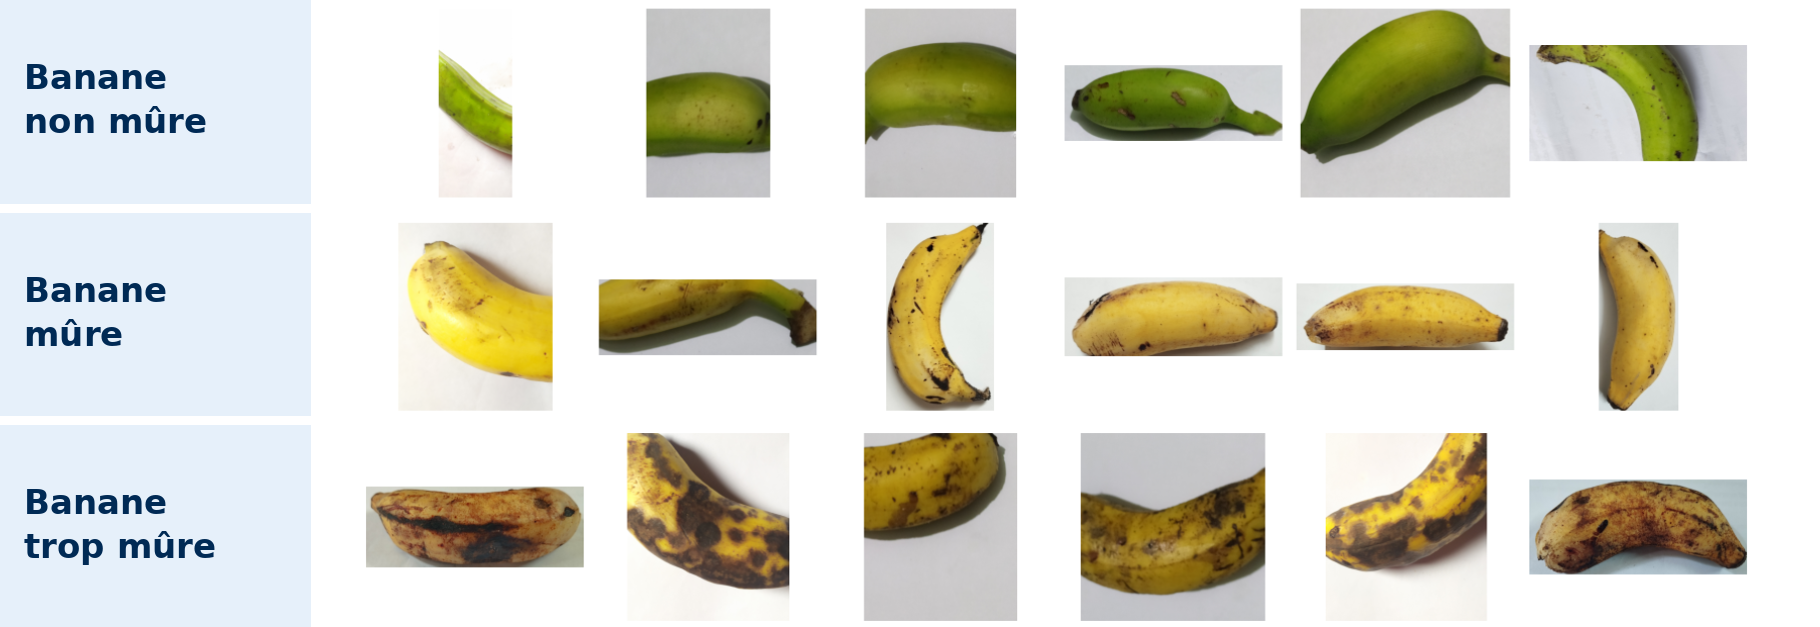
\includegraphics[width=0.9\textwidth]{figures/fig_ex_bananes.png}
\caption{Exemples de bananes recadrées, une ligne par stade de maturité.}
\end{figure}

\begin{figure}[H]
\centering
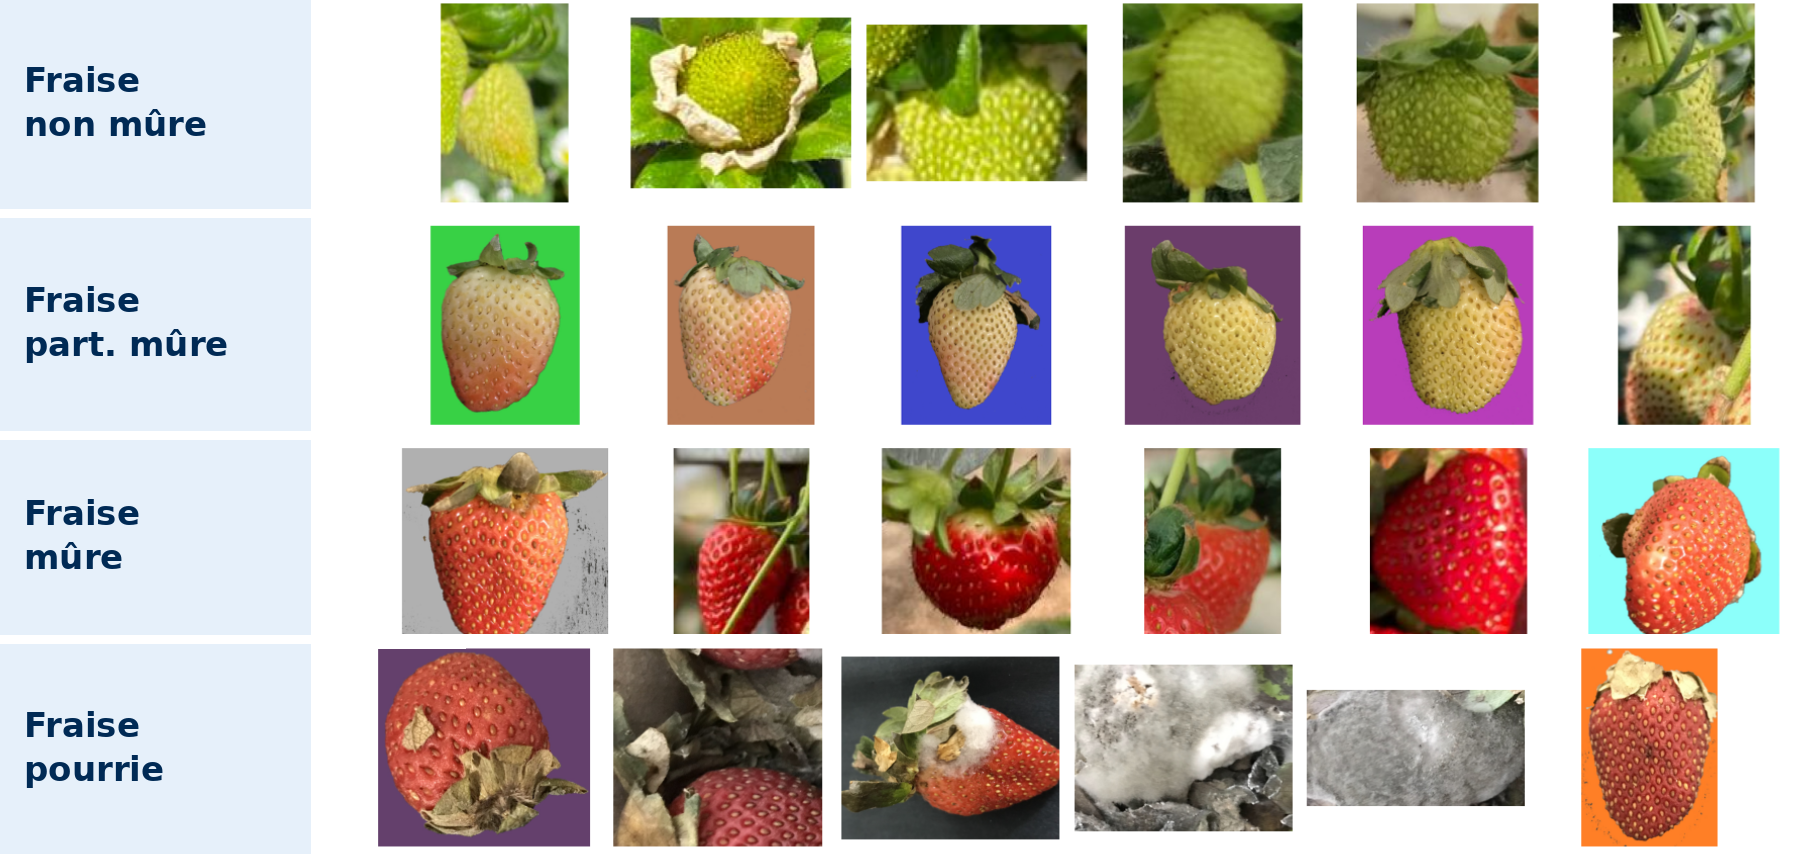
\includegraphics[width=0.9\textwidth]{figures/fig_ex_fraises.png}
\caption{Exemples de fraises recadrées, une ligne par stade, du stade non mûr au stade pourri.}
\end{figure}

\begin{figure}[H]
\centering
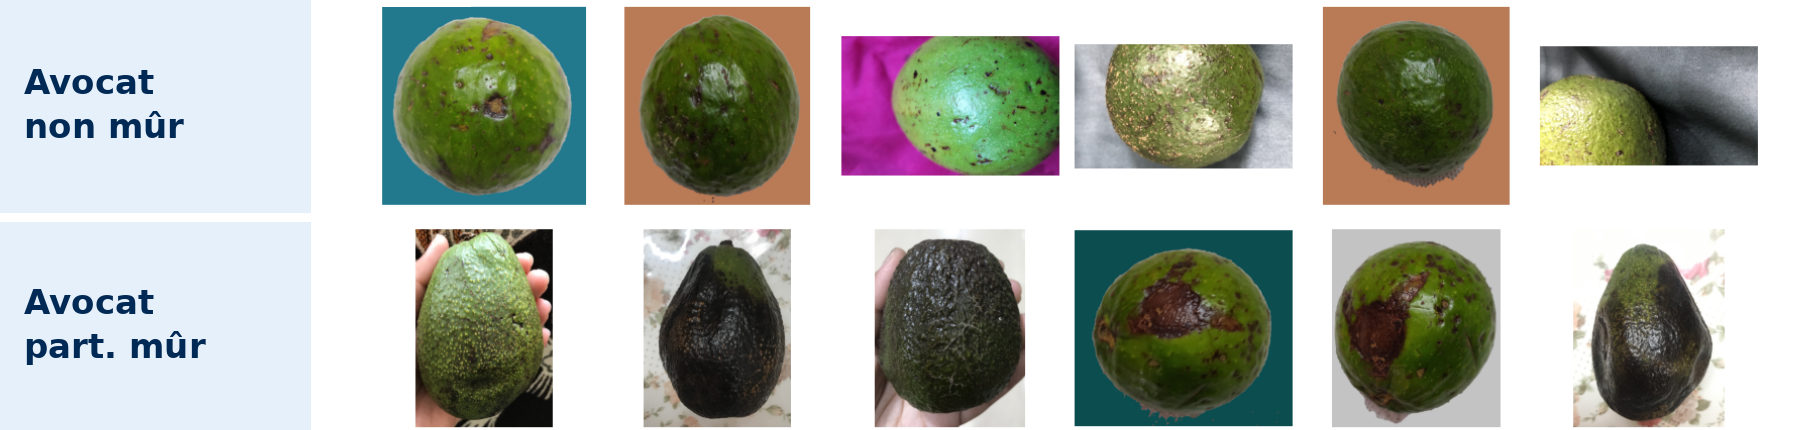
\includegraphics[width=0.9\textwidth]{figures/fig_ex_avocats.png}
\caption{Exemples d’avocats recadrés pour deux des quatre stades (non mûr et partiellement mûr).}
\end{figure}

\section{Recadrage à partir des boîtes}

Le classifieur reçoit une image d’un seul fruit. Nous recadrons donc chaque photographie selon les boîtes d’annotation. Chaque boîte YOLO est donnée par son centre $(x_c,y_c)$ et ses dimensions $(w,h)$, normalisés entre 0 et 1~; la boîte en pixels pour une image de taille $W\times H$ est~:
\begin{equation}
  x_{\min,\max} = \bigl(x_c \mp \tfrac{w’}{2}\bigr)\,W, \qquad y_{\min,\max} = \bigl(y_c \mp \tfrac{h’}{2}\bigr)\,H,
\end{equation}
avec $w’=1{,}05\,w$ et $h’=1{,}05\,h$ : nous ajoutons une \textbf{marge de 5\,\%} pour ne pas couper le bord du fruit, puis tronquons aux limites de l’image. Les boîtes de moins de \textbf{40 pixels} de côté sont ignorées, car elles ne contiennent pas assez d’information, et les recadrages sont réduits à 400 pixels maximum (miniature) pour limiter l’espace disque. Les 1\,431 photographies fournissent ainsi \textbf{1\,598 images de fruits}.

\section{Découpage sans fuite d’information}\label{sec:split}

Une même photographie peut contenir plusieurs fruits annotés. Si les recadrages d’une même photo étaient répartis entre entraînement et test, le modèle serait évalué sur des fruits voisins de ceux qu’il a vus~: c’est une \textbf{fuite d’information}, qui gonfle artificiellement la précision. Nous découpons donc \emph{par photographie d’origine} et non par recadrage~:

\begin{enumerate}
  \item chaque photo reçoit une étiquette égale à la classe majoritaire de ses boîtes~;
  \item les photos sont séparées en 70\,\% (entraînement), 15\,\% (validation) et 15\,\% (test) de façon \emph{stratifiée} sur cette étiquette, avec une graine fixée (\code{seed=42}) pour la reproductibilité ;
  \item chaque recadrage rejoint l’ensemble de sa photo.
\end{enumerate}

Le résultat est 1\,118 images d’entraînement, 249 de validation et 231 de test (tableau~\ref{tab:classes}). Le jeu de test n’est utilisé qu’à la fin pour mesurer les performances.

\begin{figure}[H]
\centering
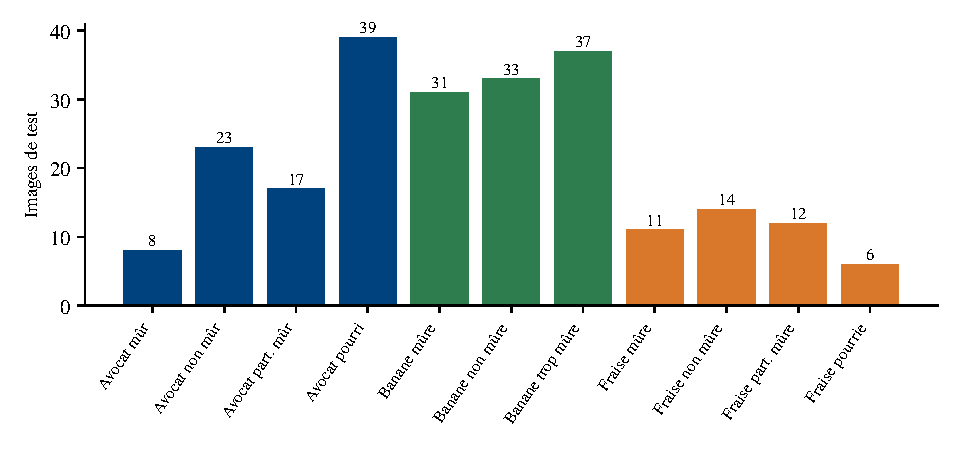
\includegraphics[width=0.78\textwidth]{figures/fig_support.pdf}
\caption{Nombre d’images de test par classe.}\label{fig:support}
\end{figure}

\section{Chaîne de chargement et prétraitement}

Les images sont lues par \code{image\_dataset\_from\_directory} de Keras, qui déduit les classes des noms de dossiers (ordre alphabétique), redimensionne à $224\times224$ pixels et forme des lots de 32 images. Les ensembles sont mis en préchargement (\code{prefetch}) pour recouvrir le calcul du GPU et le chargement des données.

Le prétraitement propre à MobileNetV2 (mise à l’échelle des pixels de $[0,255]$ vers $[-1,1]$, par une division suivie d’une soustraction) est intégré \emph{à l’intérieur du modèle}. Ce choix a un avantage décisif au déploiement~: l’application Android fournit directement les pixels bruts (valeurs 0--255) et n’a aucune normalisation à reproduire, ce qui supprime une source classique d’erreurs de décalage entre entraînement et production.

\section{Augmentation de données}

L’augmentation consiste à appliquer des transformations aléatoires aux images d’entraînement pour multiplier la diversité des exemples. Notre version retenue comprend~:

\begin{itemize}
  \item un retournement aléatoire horizontal et vertical (\code{RandomFlip})~;
  \item une rotation aléatoire jusqu’à $\pm 15\,\%$ d’un tour, soit $\pm 54^\circ$ (\code{RandomRotation})~;
  \item un zoom aléatoire de $\pm 15\,\%$ (\code{RandomZoom})~;
  \item une variation aléatoire de luminosité ($\pm 10\,\%$) et de contraste ($10\,\%$)~;
\end{itemize}

\begin{keybox}{Pas de changement de teinte}
Nous avons volontairement \emph{exclu} toute modification de la teinte (couleur)~: pour la maturité d’un fruit, la couleur est l’indice principal. Transformer du vert en jaune, ou du jaune en brun, changerait la classe de l’image sans changer son étiquette et brouillerait l’apprentissage.
\end{keybox}

Ces couches font partie du modèle mais ne sont actives qu’à l’entraînement~; la validation et le test utilisent les images telles quelles.

\section{Pondération des classes}\label{sec:poids}

Face au déséquilibre, un modèle naïf tend à favoriser les classes fréquentes. Nous attribuons à chaque classe un poids $\omega_k$ inversement proportionnel à sa fréquence, selon la formule «~balanced~» de scikit-learn~:
\begin{equation}
  \omega_k = \frac{N}{K\cdot n_k},
\end{equation}
où $N=1\,118$ est le nombre d’images d’entraînement, $K=11$ le nombre de classes et $n_k$ l’effectif de la classe $k$. Une erreur sur une classe rare coûte donc plus cher dans la perte. Les poids obtenus vont de \textbf{0,56} (avocat pourri, la plus fréquente) à \textbf{3,08} (avocat mûr, la plus rare)~; les trois classes de bananes, nombreuses, ont des poids compris entre 0,58 et 0,71.

\begin{table}[H]
\centering
\caption{Poids de classes utilisés dans la perte.}\label{tab:poids}
\small
\begin{tabular}{@{}lrlr@{}}
\toprule
\textbf{Classe} & $\omega_k$ & \textbf{Classe} & $\omega_k$ \\
\midrule
avocat mûr & 3,08 & banane mûre & 0,71 \\
fraise mûre & 2,12 & banane non mûre & 0,66 \\
fraise partiellement mûre & 1,85 & banane trop mûre & 0,58 \\
fraise pourrie & 1,49 & avocat non mûr & 0,93 \\
fraise non mûre & 1,39 & avocat pourri & 0,56 \\
avocat partiellement mûr & 1,30 & & \\
\bottomrule
\end{tabular}
\end{table}

Cette pondération améliore le rappel des classes rares au prix d’une légère baisse de précision sur les classes fréquentes, compromis jugé acceptable~: une fraise mûre manquée est plus gênante qu’une hésitation sur une banane.

\chapter{Modèle et entraînement}\label{chap:modele}

Ce chapitre décrit l’architecture complète du classifieur, la procédure d’entraînement en deux phases et les choix d’hyperparamètres. Le code correspondant est donné en annexe~\ref{app:code}.

\section{Architecture du modèle}

Le modèle enchaîne cinq blocs, de l’image brute aux probabilités (figure~\ref{fig:modele})~:

\begin{enumerate}
  \item l’\textbf{entrée}~: une image $224\times224\times3$ dont les pixels sont des flottants entre 0 et 255~;
  \item le bloc d’\textbf{augmentation} (retournements, rotation, zoom, luminosité, contraste), actif seulement à l’entraînement~;
  \item le \textbf{prétraitement} MobileNetV2~: division par 127,5 puis soustraction de 1, pour obtenir des valeurs dans $[-1,1]$ ;
  \item la \textbf{base MobileNetV2} pré-entraînée sur ImageNet, sans sa tête, qui produit une carte de caractéristiques $7\times7\times1280$ ;
  \item la \textbf{tête de classification}~: pooling moyen global ($1280$ valeurs), dropout de taux $0{,}3$, couche dense à 11 sorties avec softmax.
\end{enumerate}

\begin{figure}[H]
\centering
\begin{tikzpicture}[node distance=3mm]
  \node[blkw,minimum width=19mm,minimum height=17mm] (a) {\textbf{Image}\\[-1pt]\scriptsize $224{\times}224{\times}3$\\0--255};
  \node[blko,minimum width=21mm,minimum height=17mm,right=of a] (b) {\textbf{Augmen-}\\\textbf{tation}\\[-1pt]{\scriptsize (train seul.)}};
  \node[blk,minimum width=19mm,minimum height=17mm,right=of b] (c) {\textbf{Prétrait.}\\[-1pt]{\scriptsize $[-1,1]$}};
  \node[blk,minimum width=24mm,minimum height=17mm,right=of c,fill=navy!14] (d) {\textbf{MobileNetV2}\\[-1pt]\scriptsize $7{\times}7{\times}1280$\\2\,257\,984 param.};
  \node[blk,minimum width=21mm,minimum height=17mm,right=of d] (e) {\textbf{GAP +}\\\textbf{Dropout 0,3}\\[-1pt]{\scriptsize 1280}};
  \node[blkg,minimum width=21mm,minimum height=17mm,right=of e] (f) {\textbf{Dense 11}\\[-1pt]\scriptsize softmax\\14\,091 param.};
  \foreach \x/\y in {a/b,b/c,c/d,d/e,e/f} \draw[arr] (\x) -- (\y);
\end{tikzpicture}
\caption{Architecture complète du classifieur de maturité.}\label{fig:modele}
\end{figure}

\paragraph{Nombre de paramètres.} La tête contient $1280\times 11 + 11 = 14\,091$ paramètres (poids plus biais). Ajoutée aux $2\,257\,984$ paramètres de la base, elle porte le total à \textbf{2\,272\,075} paramètres. Plus de 99\,\% du modèle provient donc de la base pré-entraînée.

\begin{table}[H]
\centering
\caption{Répartition des paramètres.}\label{tab:params}
\small
\begin{tabular}{@{}lrr@{}}
\toprule
\textbf{Partie} & \textbf{Paramètres} & \textbf{Part} \\
\midrule
Base MobileNetV2 (sans tête) & 2\,257\,984 & 99,4\,\% \\
Tête (dense $1280\to 11$) & 14\,091 & 0,6\,\% \\
\midrule
\textbf{Total} & \textbf{2\,272\,075} & 100\,\% \\
\bottomrule
\end{tabular}
\end{table}

\section{Fonction de perte et métrique}

La perte est l’\textbf{entropie croisée catégorielle} (chapitre~\ref{chap:dl}), calculée sur les étiquettes entières (\code{sparse\_categorical\_crossentropy}) et pondérée par les poids de classes de la section~\ref{sec:poids}. La métrique suivie pendant l’entraînement est l’exactitude (proportion d’images correctement classées).

\section{Phase 1~: entraînement de la tête}

Dans la première phase, la base MobileNetV2 est \textbf{gelée}~: ses poids ne changent pas. Seule la tête de 14\,091 paramètres est entraînée. Les caractéristiques extraites par la base sont déjà très riches~; la tête apprend simplement à les combiner pour reconnaître nos 11 classes.

\begin{itemize}
  \item optimiseur \textbf{Adam}, taux d’apprentissage $10^{-3}$ ;
  \item au plus \textbf{25 époques}, lots de 32 images~;
  \item \textbf{EarlyStopping} sur la perte de validation (patience 6), avec restauration des meilleurs poids~;
  \item \textbf{ReduceLROnPlateau}~: le taux est divisé par deux si la perte de validation stagne pendant 3 époques.
\end{itemize}

Le gel de la base est cohérent avec la logique du transfert~: avec un taux élevé, des gradients issus d’une tête initialisée au hasard abîmeraient les poids pré-entraînés. La phase 1 se termine après une douzaine d’époques, avec une exactitude de validation d’environ 91\,\%.

\section{Phase 2~: fine-tuning}\label{sec:finetune}

Dans la deuxième phase, nous \textbf{dégelons les 40 dernières couches} de la base et continuons l’entraînement avec un taux d’apprentissage beaucoup plus faible, afin d’adapter finement les caractéristiques de haut niveau aux fruits sans détruire ce qui a été appris sur ImageNet.

\begin{itemize}
  \item optimiseur Adam, taux d’apprentissage \textbf{$10^{-5}$} (cent fois plus faible)~;
  \item au plus \textbf{40 époques}~;
  \item EarlyStopping sur la perte de validation (patience 10) et ReduceLROnPlateau (facteur 0,5, patience 4, taux minimal $10^{-7}$)~;
  \item \textbf{couches de normalisation par lots gelées}~: parmi les couches dégelées, les couches BatchNormalization restent figées.
\end{itemize}

\begin{keybox}{Pourquoi geler la BatchNormalization~?}
Ces couches maintiennent des moyennes et variances mobiles calculées sur ImageNet. En fine-tuning sur un petit jeu de données et de petits lots, mettre à jour ces statistiques les rend instables et dégrade la précision. Les laisser figées est la pratique recommandée par la documentation de Keras, et cette précaution, associée à la correction des callbacks décrite plus bas, a fait passer notre exactitude de test de 90,0\,\% à 93,1\,\% (chapitre~\ref{chap:resultats}, expériences 1 et 2).
\end{keybox}

\section{Courbes d’apprentissage}

La figure~\ref{fig:courbes} montre l’évolution de l’exactitude et de la perte au fil des époques. L’exactitude de validation monte rapidement pendant la phase 1 (environ 91\,\%), puis progresse plus lentement pendant le fine-tuning pour se stabiliser autour de 92\,\%. L’exactitude d’entraînement atteint environ 97\,\%.

\begin{figure}[H]
\centering
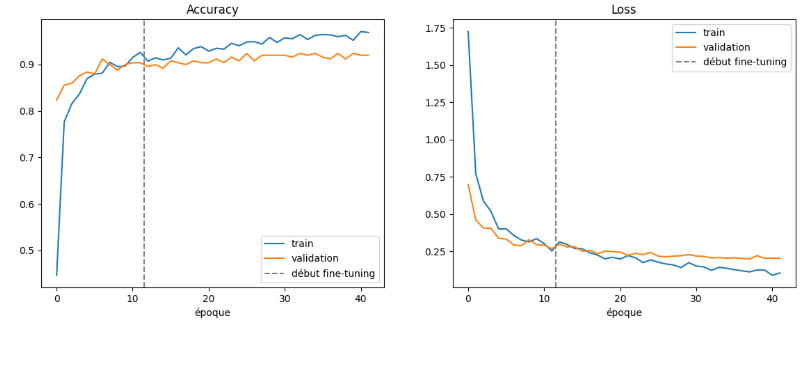
\includegraphics[width=0.96\textwidth]{figures/courbes.png}
\caption{Courbes d’apprentissage~: exactitude et perte, entraînement et validation, phases 1 et 2.}\label{fig:courbes}
\end{figure}

\paragraph{Lecture.} L’écart d’environ cinq points entre l’entraînement (97\,\%) et la validation (92\,\%) indique un \textbf{surapprentissage modéré} : le modèle s’adapte un peu mieux aux images qu’il a vues qu’aux nouvelles. Il n’est pas catastrophique, car la perte de validation ne remonte pas, et il est atténué par l’arrêt anticipé et le dropout. Avec seulement 1\,118 images d’entraînement, il est difficile de le réduire davantage sans nouvelles données.

\section{Hyperparamètres retenus}

\begin{table}[H]
\centering
\caption{Récapitulatif de la configuration de l’entraînement.}\label{tab:hyper}
\small
\begin{tabular}{@{}p{5.2cm}p{4.5cm}p{3.8cm}@{}}
\toprule
\textbf{Paramètre} & \textbf{Phase 1} & \textbf{Phase 2} \\
\midrule
Couches entraînées & Tête uniquement & 40 dernières couches de la base + tête (BatchNorm gelées) \\
Optimiseur & Adam & Adam \\
Taux d’apprentissage & $10^{-3}$ & $10^{-5}$ \\
Époques maximales & 25 & 40 \\
Taille de lot & 32 & 32 \\
EarlyStopping (val\_loss) & patience 6 & patience 10 \\
ReduceLROnPlateau & ×0,5, patience 3 & ×0,5, patience 4 \\
Dropout & 0,3 & 0,3 \\
Poids de classes & \multicolumn{2}{c}{«~balanced~» (0,56 à 3,08)} \\
Entrée & \multicolumn{2}{c}{$224\times224\times3$, pixels 0--255} \\
\bottomrule
\end{tabular}
\end{table}

\section{Un piège rencontré~: la réutilisation des callbacks}

Notre première tentative a donné 90,0\,\%. Deux corrections ont ensuite été apportées. D’abord, les mêmes objets \code{callbacks} avaient été réutilisés dans les deux phases ; or EarlyStopping conserve en mémoire la meilleure valeur observée et son compteur de patience. En phase 2, il comparait la perte de validation à la meilleure valeur de la phase 1 et pouvait donc stopper l’entraînement trop tôt. Nous créons maintenant de nouveaux objets pour chaque phase. Ensuite, nous avons gelé les couches BatchNormalization pendant le fine-tuning (encadré précédent). Ces deux corrections ont donné le modèle retenu à 93,1\,\%.

\section{Environnement de calcul}

L’entraînement a été exécuté sur Kaggle avec deux GPU NVIDIA T4. Une époque dure environ 3 à 4 secondes (environ 35 lots de 32 images), si bien que la procédure complète tient en quelques minutes. Cette rapidité permet d’explorer plusieurs variantes, comme nous l’avons fait au chapitre suivant.

\chapter{Évaluation et résultats}\label{chap:resultats}

Ce chapitre présente les performances du modèle sur le jeu de test (231 images jamais vues pendant l’entraînement ni le choix des hyperparamètres), analyse ses erreurs et décrit les expériences complémentaires qui ont guidé nos choix.

\section{Métriques d’évaluation}

Soit $TP_k$, $FP_k$ et $FN_k$ les vrais positifs, faux positifs et faux négatifs de la classe $k$. On définit~:
\begin{align}
  \text{exactitude} &= \frac{\text{prédictions correctes}}{\text{nombre total d’images}}, \\
  \text{précision}_k &= \frac{TP_k}{TP_k+FP_k}, \qquad
  \text{rappel}_k = \frac{TP_k}{TP_k+FN_k}, \\
  F1_k &= \frac{2\cdot \text{précision}_k\cdot\text{rappel}_k}{\text{précision}_k+\text{rappel}_k}.
\end{align}
La \textbf{précision} d’une classe répond à «~quand le modèle annonce cette classe, a-t-il raison~?~» et le \textbf{rappel} à «~parmi les vraies images de cette classe, combien sont retrouvées~?~». Le score F1 est leur moyenne harmonique. La \textbf{moyenne macro} calcule la moyenne simple de ces valeurs sur les 11 classes, sans tenir compte des effectifs~: elle est donc sensible aux classes rares, contrairement à l’exactitude.

\section{Résultats globaux}

Sur les 231 images de test, le modèle classe correctement 215, soit une \textbf{exactitude de 93,1\,\%}. Les moyennes macro sont une précision de 0,910, un rappel de 0,895 et un score F1 de 0,897. L’écart entre l’exactitude et la moyenne macro (environ trois points) reflète le fait que les classes rares sont un peu moins bien reconnues que les classes fréquentes.

\paragraph{Intervalle de confiance.} Avec 231 images de test, l’exactitude mesurée est elle-même incertaine. L’intervalle de Wilson à 95\,\% pour 215 réussites sur 231 essais est \textbf{[89,0\,\% ; 95,7\,\%]}. Il faut donc lire « environ 93\,\% » et non voir dans la décimale une garantie ; deux modèles dont les exactitudes diffèrent d’un ou deux points ne sont pas statistiquement distinguables sur ce test.

\section{Résultats par fruit}

\begin{table}[H]
\centering
\caption{Exactitude par fruit sur le jeu de test.}\label{tab:fruit}
\small
\begin{tabular}{@{}lrrr@{}}
\toprule
\textbf{Fruit} & \textbf{Images} & \textbf{Correctes} & \textbf{Exactitude} \\
\midrule
Banane & 101 & 99 & 98,0\,\% \\
Avocat & 87 & 81 & 93,1\,\% \\
Fraise & 43 & 35 & 81,4\,\% \\
\midrule
\textbf{Total} & \textbf{231} & \textbf{215} & \textbf{93,1\,\%} \\
\bottomrule
\end{tabular}
\end{table}

Les bananes sont presque parfaitement classées~: leurs trois stades ont des couleurs franches (vert, jaune, jaune tacheté de brun). Les fraises sont les plus difficiles~: c’est le fruit qui compte le moins d’images et dont les stades intermédiaires (rouge clair, rouge mûr) se ressemblent le plus.

\section{Résultats par classe}

\begin{table}[H]
\centering
\caption{Précision, rappel et F1 par classe sur le jeu de test.}\label{tab:classe}
\small
\begin{tabular}{@{}lrrrr@{}}
\toprule
\textbf{Classe} & \textbf{Précision} & \textbf{Rappel} & \textbf{F1} & \textbf{Support} \\
\midrule
Avocat mûr & 1,00 & 0,88 & 0,93 & 8 \\
Avocat non mûr & 0,95 & 0,83 & 0,88 & 23 \\
Avocat partiellement mûr & 0,80 & 0,94 & 0,86 & 17 \\
Avocat pourri & 0,97 & 1,00 & 0,99 & 39 \\
Banane mûre & 0,97 & 0,97 & 0,97 & 31 \\
Banane non mûre & 1,00 & 1,00 & 1,00 & 33 \\
Banane trop mûre & 0,97 & 0,97 & 0,97 & 37 \\
Fraise mûre & 0,63 & 0,91 & 0,74 & 11 \\
Fraise non mûre & 1,00 & 0,86 & 0,92 & 14 \\
Fraise partiellement mûre & 0,89 & 0,67 & 0,76 & 12 \\
Fraise pourrie & 0,83 & 0,83 & 0,83 & 6 \\
\midrule
\textbf{Moyenne macro} & \textbf{0,910} & \textbf{0,895} & \textbf{0,897} & 231 \\
\bottomrule
\end{tabular}
\end{table}

\begin{figure}[H]
\centering
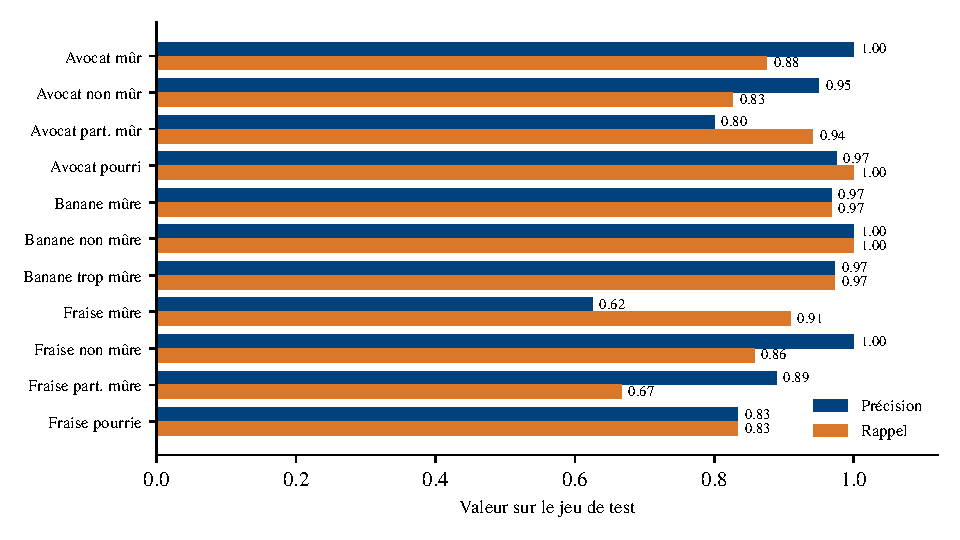
\includegraphics[width=0.95\textwidth]{figures/fig_prf.pdf}
\caption{Précision, rappel et F1 par classe.}\label{fig:prf}
\end{figure}

La «~fraise pourrie~» n’a que 6 images de test~: une seule erreur fait varier son rappel de 17 points. Les valeurs sur les classes de fraises et sur «~avocat mûr~» (8 images) doivent donc être interprétées avec prudence.

\section{Matrice de confusion}

La matrice de confusion (figure~\ref{fig:confusion}) compte, pour chaque classe réelle (lignes), les classes prédites (colonnes). La diagonale correspond aux bonnes réponses.

\begin{figure}[H]
\centering
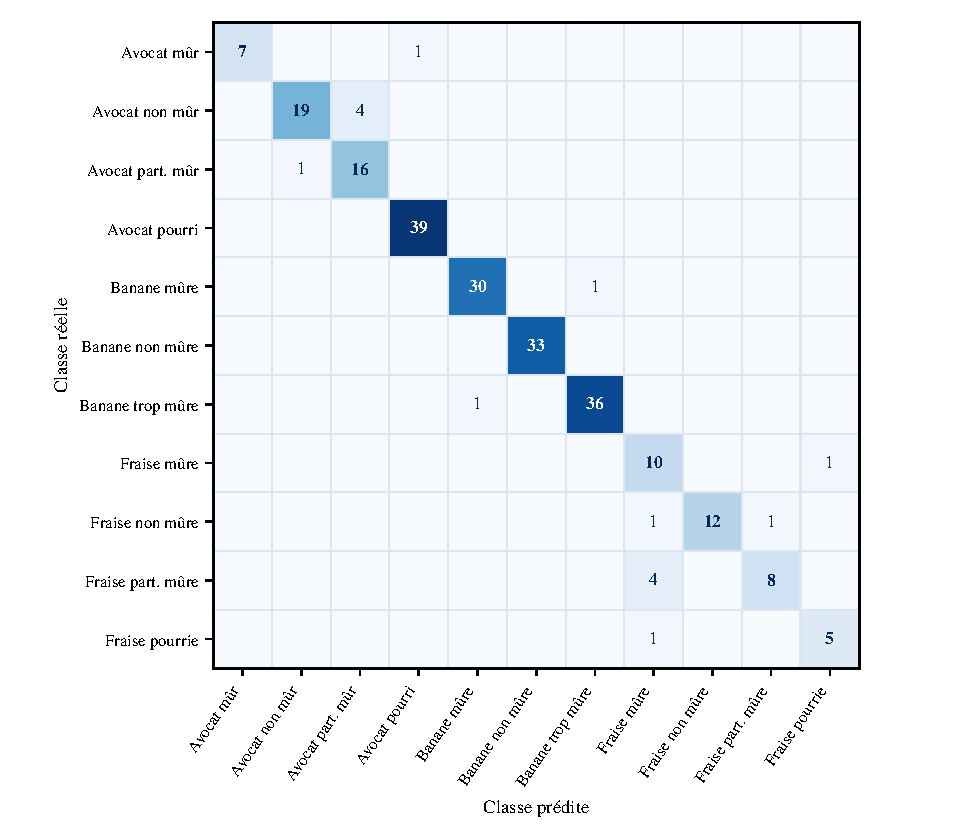
\includegraphics[width=0.92\textwidth]{figures/fig_confusion.pdf}
\caption{Matrice de confusion sur le jeu de test (231 images).}\label{fig:confusion}
\end{figure}

Le modèle commet \textbf{16 erreurs}. Elles sont toutes concentrées entre des stades \emph{voisins} du même fruit, ou entre «~mûr~» et «~pourri~»~:

\begin{table}[H]
\centering
\caption{Inventaire des 16 erreurs de classification.}\label{tab:erreurs}
\small
\begin{tabular}{@{}llr@{}}
\toprule
\textbf{Classe réelle} & \textbf{Classe prédite} & \textbf{Nombre} \\
\midrule
Avocat non mûr & Avocat partiellement mûr & 4 \\
Fraise partiellement mûre & Fraise mûre & 4 \\
Avocat mûr & Avocat pourri & 1 \\
Avocat partiellement mûr & Avocat non mûr & 1 \\
Banane mûre & Banane trop mûre & 1 \\
Banane trop mûre & Banane mûre & 1 \\
Fraise mûre & Fraise pourrie & 1 \\
Fraise non mûre & Fraise mûre & 1 \\
Fraise non mûre & Fraise partiellement mûre & 1 \\
Fraise pourrie & Fraise mûre & 1 \\
\midrule
\textbf{Total} & & \textbf{16} \\
\bottomrule
\end{tabular}
\end{table}

\paragraph{Analyse.} Aucune confusion ne mélange deux fruits différents~: l’identification du fruit est donc fiable à 100\,\% sur ce test. Toutes les erreurs portent sur le stade de maturité. Huit des seize erreurs relèvent de deux familles bien identifiées :

\begin{itemize}
  \item les \textbf{avocats non mûrs pris pour partiellement mûrs} (4 cas), et les \textbf{fraises partiellement mûres prises pour mûres} (4 cas). Dans les deux cas, le modèle choisit le stade voisin~: la maturité est un continuum et la frontière entre deux classes est floue, y compris pour un annotateur humain~;
  \item quelques erreurs isolées entre stades adjacents (banane mûre/trop mûre, fraise non mûre/mûre).
\end{itemize}

Ces erreurs sont de faible gravité pratique, puisque l’utilisateur n’est jamais induit en erreur sur le fruit et se trompe rarement de plus d’un cran de maturité. L’erreur la plus sérieuse est «~avocat mûr prédit pourri~» (1 cas), qui pourrait conduire à jeter un fruit consommable.

\section{Expériences complémentaires}

Pour évaluer la robustesse de nos choix, nous avons mené plusieurs variantes d’entraînement. Elles diffèrent par la configuration, mais pas par le jeu de test, sauf la dernière (tableau~\ref{tab:exp}).

\begin{table}[H]
\centering
\caption{Résumé des expériences et exactitudes sur le jeu de test.}\label{tab:exp}
\small
\begin{tabularx}{\textwidth}{@{}lXr@{}}
\toprule
\textbf{N°} & \textbf{Configuration} & \textbf{Exactitude} \\
\midrule
1 & Première version, callbacks réutilisés entre les deux phases & 90,0\,\% \\
2 & Callbacks recréés, BatchNorm gelées (\textbf{modèle retenu}) & \textbf{93,1\,\%} \\
3 & Augmentation renforcée (rotation 0,2, translation, bruit gaussien, dropout 0,4, 60 couches dégelées) & 90,9\,\% \\
4 & Ajout de 624 images de bananes d’une autre source (test de 352 images) & 86,6\,\% \\
\bottomrule
\end{tabularx}
\end{table}

\begin{figure}[H]
\centering
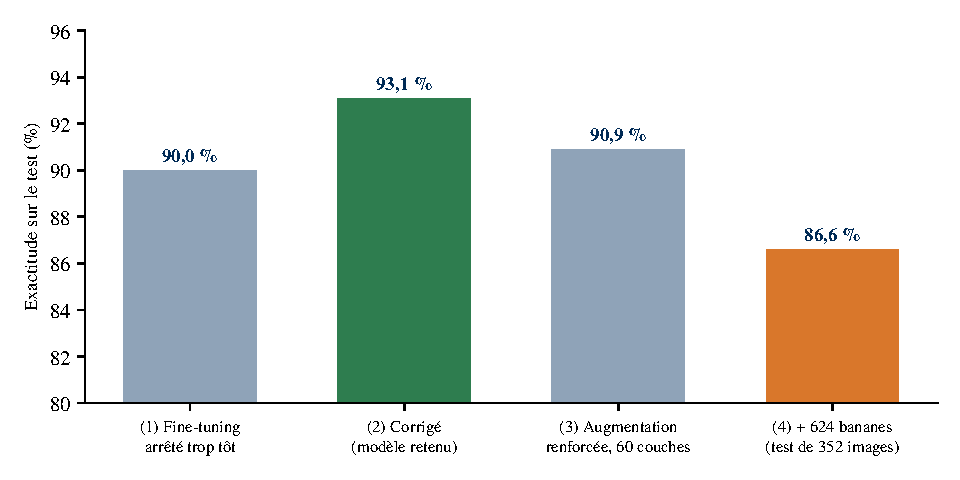
\includegraphics[width=0.78\textwidth]{figures/fig_experiences.pdf}
\caption{Exactitude de test des quatre expériences.}\label{fig:exp}
\end{figure}

\paragraph{Expérience 3~: augmenter plus fort n’aide pas.} Avec une augmentation plus agressive (retournement vertical, rotation jusqu’à 20\,\%, translation, bruit gaussien, dropout de 0,4) et 60 couches dégelées, l’exactitude tombe à 90,9\,\% (91,3\,\% après conversion TFLite). Avec 1\,118 images, des transformations trop fortes déforment les fruits au point de brouiller les indices utiles. La différence avec le modèle retenu (2,2 points) reste dans l’intervalle d’incertitude du test, mais aucune amélioration n’est observée ; nous conservons donc la configuration la plus simple.

\paragraph{Expérience 4~: plus de données, mais d’une autre origine.} Nous avons ajouté 624 images de bananes issues d’un jeu externe (collecte web, préfixe \code{web\_}), réparties en 432 images d’entraînement, 96 de validation et 96 de test, ce qui porte les ensembles à 1\,517, 353 et 352 images. L’exactitude globale baisse à 86,6\,\% : sur les 96 images \code{web\_}, elle n’est que de 80,2\,\%, contre 89,1\,\% sur le reste du test. Le rappel de « banane trop mûre » tombe à 0,68.

L’explication la plus plausible est une \textbf{incohérence d’étiquetage} entre les sources~: ce qu’un annotateur appelle «~trop mûre~» n’est pas ce qu’un autre appelle ainsi, et les bananes web ont des conditions de prise de vue différentes. C’est une leçon importante~: \emph{ajouter des données n’améliore le modèle que si elles sont étiquetées selon la même convention}. Nous n’avons pas retenu cette variante.

\section{Synthèse}

\begin{keybox}{Ce qu’il faut retenir}
\begin{itemize}[leftmargin=*,itemsep=2pt]
  \item Exactitude de test~: \textbf{93,1\,\%} (IC à 95\,\% : 89,0--95,7\,\%), F1 macro 0,897.
  \item Le fruit est toujours bien identifié~; les erreurs portent sur des stades voisins.
  \item Les bananes sont presque parfaites (98\,\%), les fraises les moins bien reconnues (81\,\%).
  \item Plus de données ou plus d’augmentation n’ont pas amélioré le modèle~: la qualité et la cohérence des étiquettes comptent plus que la quantité.
\end{itemize}
\end{keybox}

\chapter{Conversion TensorFlow Lite et quantification}\label{chap:tflite}

Le modèle Keras produit à l’issue de l’entraînement occupe plus de 23\,Mo et dépend de la bibliothèque TensorFlow complète. Pour l’embarquer sur un téléphone, nous le convertissons au format \textbf{TensorFlow Lite} (TFLite), conçu pour les appareils mobiles, puis nous le \textbf{quantifions} pour réduire encore sa taille.

\section{Le format TensorFlow Lite}

Un fichier \code{.tflite} est un graphe de calcul sérialisé au format FlatBuffers~: il contient les opérations du réseau et les poids dans un seul fichier compact, qui peut être lu sans copie en mémoire. Il est exécuté par un \emph{interpréteur} très léger, disponible pour Android, iOS et les microcontrôleurs, qui sélectionne les opérations optimisées pour le processeur de l’appareil. Le modèle ne dépend plus ni de Python ni de Keras.

\section{La quantification}

Les poids d’un réseau sont stockés en nombres flottants sur 32 bits. La \textbf{quantification} les représente sur moins de bits, typiquement des entiers sur 8 bits~\cite{jacob2018}. Chaque valeur réelle $x$ est approchée par un entier $q\in[-128,127]$ à l’aide d’un facteur d’échelle $s$ et d’un décalage $z$ :
\begin{equation}
  x \approx s\,(q - z), \qquad q = \operatorname{round}\!\left(\frac{x}{s}\right)+z.
\end{equation}
Le facteur $s$ est calculé par tenseur (ou par canal), en fonction de l’étendue des valeurs à représenter. Passer de 32 à 8 bits divise l’espace occupé par quatre, au prix d’une petite erreur d’arrondi sur chaque poids.

Nous utilisons la \textbf{quantification dynamique} (\emph{dynamic range quantization})~: seuls les \emph{poids} sont stockés en 8 bits~; les activations restent en flottant et sont quantifiées à la volée pendant l’inférence. C’est la variante la plus simple (option \code{DEFAULT} du convertisseur), qui ne demande aucune image de calibration.

\section{Procédure de conversion}

La conversion se fait en quelques lignes à partir du modèle Keras entraîné~:

\begin{lstlisting}[language=PythonK]
converter = tf.lite.TFLiteConverter.from_keras_model(model)
converter.optimizations = [tf.lite.Optimize.DEFAULT]   # poids en 8 bits
tflite_model = converter.convert()
open("fruit_ripeness.tflite", "wb").write(tflite_model)
\end{lstlisting}

Comme le prétraitement est inclus dans le modèle (chapitre~\ref{chap:modele}), le fichier produit a l’interface suivante~:

\begin{table}[H]
\centering
\caption{Interface du modèle TFLite.}\label{tab:io}
\small
\begin{tabular}{@{}lll@{}}
\toprule
 & \textbf{Forme} & \textbf{Contenu} \\
\midrule
Entrée & $[1,224,224,3]$, \code{float32} & Pixels RGB entre 0 et 255 \\
Sortie & $[1,11]$, \code{float32} & Probabilités softmax des 11 classes \\
\bottomrule
\end{tabular}
\end{table}

L’ordre des 11 sorties est l’ordre alphabétique des noms de classes, enregistré dans le fichier \code{labels.txt} livré avec l’application. Une inversion de cet ordre produirait des résultats absurdes mais sans message d’erreur~: le fichier d’étiquettes doit toujours être généré par le même carnet que le modèle.

\section{Effets de la quantification}

Nous avons comparé le modèle Keras (flottants 32 bits) et le modèle TFLite quantifié sur les mêmes 231 images de test.

\begin{table}[H]
\centering
\caption{Comparaison du modèle Keras et du modèle TFLite quantifié.}\label{tab:quant}
\small
\begin{tabular}{@{}lrr@{}}
\toprule
 & \textbf{Keras (float32)} & \textbf{TFLite (poids 8 bits)} \\
\midrule
Taille du fichier & 23,1\,Mo & \textbf{2,5\,Mo} \\
Exactitude de test & 93,07\,\% (215/231) & 92,64\,\% (214/231) \\
Prédictions identiques & \multicolumn{2}{c}{99,6\,\% (230 images sur 231)} \\
Temps d’inférence moyen (CPU Kaggle) & --- & 19,6\,ms par image \\
\bottomrule
\end{tabular}
\end{table}

La taille est divisée par \textbf{9} environ, pour une perte d’une seule image correctement classée sur 231 (0,43 point), bien en dessous de l’incertitude de la mesure. Le modèle quantifié donne la même réponse que le modèle d’origine dans 230 cas sur 231. La quantification est donc quasi sans perte ici~; elle est essentielle pour un téléchargement rapide et un faible encombrement mémoire.

\begin{defbox}{D’où vient la différence de taille~?}
Les 2,27 millions de paramètres occupent environ 9\,Mo en 32 bits, contre environ 2,3\,Mo en 8 bits ($2{,}27\cdot10^6 \times 1\ \text{octet}$), ce qui explique l’essentiel des 2,5\,Mo du fichier TFLite. Le fichier Keras de 23,1\,Mo est plus volumineux que les seuls poids, car il enregistre aussi des variables utiles à l’entraînement (notamment l’état de l’optimiseur) et la description complète du modèle~; le fichier TFLite ne garde que ce qui sert à l’inférence.
\end{defbox}

\section{Temps d’inférence}

Sur le CPU d’un carnet Kaggle, le modèle quantifié met en moyenne 19,6\,ms par image. Sur l’émulateur Android (processeur émulé, plus lent), les temps mesurés dans l’application sont de 46 à 380\,ms par photo, car chaque prédiction exécute le réseau \emph{deux fois} (image puis son miroir, section~\ref{sec:tta}). Ces valeurs restent très inférieures à la seconde. Sur un vrai téléphone, le temps devrait être comparable ou meilleur, mais nous ne l’avons pas mesuré faute d’appareil physique.

\chapter{Application Android}\label{chap:android}

Ce chapitre décrit l’application qui embarque le modèle~: son architecture, la chaîne de traitement d’une photo, la logique de décision (seuil de confiance et conseils) et les tests effectués.

\section{Cahier des charges de l’application}

L’application doit~: (i) permettre de prendre une photo ou d’en choisir une dans la galerie~; (ii) identifier le fruit et son stade de maturité \emph{localement}, sans connexion~; (iii) afficher le résultat de façon lisible, avec le niveau de confiance et des probabilités alternatives~; (iv) éviter de présenter comme certain un résultat que le modèle ne maîtrise pas~; (v) donner un conseil pratique adapté au stade détecté.

\section{Architecture}

L’application est écrite en \textbf{Kotlin} et comporte une seule activité (\code{MainActivity}). L’interface est décrite en XML avec des composants Material 3 (cartes, boutons, indicateurs de progression linéaires). Le modèle \code{fruit\_ripeness.tflite} et le fichier \code{labels.txt} sont placés dans le dossier \code{assets}, et sont chargés au démarrage. La bibliothèque TensorFlow Lite (version 2.17.0) fournit l’interpréteur.

\begin{figure}[H]
\centering
\begin{tikzpicture}[node distance=5mm]
  \node[blkw,minimum width=28mm,minimum height=15mm] (u) {\textbf{Utilisateur}\\[-1pt]{\footnotesize photo ou galerie}};
  \node[blk,minimum width=30mm,minimum height=15mm,right=of u] (d) {\textbf{Décodage}\\[-1pt]\footnotesize ImageDecoder\\orientation EXIF};
  \node[blk,minimum width=30mm,minimum height=15mm,right=of d] (p) {\textbf{Prétraitement}\\[-1pt]\footnotesize $224{\times}224$, RGB\\float32 0--255};
  \node[blk,minimum width=30mm,minimum height=15mm,below=7mm of p,fill=navy!14] (m) {\textbf{Interpréteur TFLite}\\[-1pt]{\footnotesize image + miroir}};
  \node[blk,minimum width=30mm,minimum height=15mm,left=of m] (a) {\textbf{Moyenne (TTA)}\\[-1pt]{\footnotesize 11 probabilités}};
  \node[blkg,minimum width=28mm,minimum height=15mm,left=of a] (r) {\textbf{Affichage}\\[-1pt]\footnotesize résultat, conseil,\\top-3};
  \draw[arr] (u) -- (d); \draw[arr] (d) -- (p); \draw[arr] (p) -- (m); \draw[arr] (m) -- (a); \draw[arr] (a) -- (r);
\end{tikzpicture}
\caption{Chaîne de traitement d’une photo dans l’application.}\label{fig:android}
\end{figure}

\section{Acquisition de l’image}

\begin{itemize}
  \item \textbf{Galerie}~: le sélecteur système \code{PickVisualMedia} permet de choisir une image sans demander aucune permission de stockage.
  \item \textbf{Appareil photo}~: l’application demande à l’appareil photo du système d’écrire une photo en \emph{pleine résolution} dans un fichier privé, via un \code{FileProvider}. L’option plus simple \code{TakePicturePreview} ne renvoie qu’une miniature de faible résolution, trop pauvre pour juger la couleur et la texture d’un fruit~; nous l’avons donc écartée.
\end{itemize}

\section{Décodage et prétraitement}

L’image est décodée avec \code{ImageDecoder}, qui applique automatiquement l’orientation EXIF~: une photo prise en portrait n’est pas affichée ni analysée de travers. L’image est limitée à 1\,024 pixels sur son plus grand côté (constante \code{MAX\_DISPLAY}) pour limiter la mémoire. Elle est ensuite redimensionnée à $224\times224$ et convertie en tableau de flottants~: pour chaque pixel, les valeurs R, G, B entre 0 et 255 sont écrites dans l’ordre dans un tampon de $224\times224\times3\times4$ octets. Aucune normalisation n’est nécessaire côté Kotlin, car elle est incluse dans le modèle.

Le décodage et l’inférence s’exécutent dans un \emph{thread} séparé afin de ne pas bloquer l’interface~; le résultat est publié sur le thread principal. Un indicateur de chargement est affiché entre-temps.

\section{Test-time augmentation (TTA)}\label{sec:tta}

Pour stabiliser les prédictions, l’application classe l’image \emph{et son miroir horizontal}, puis fait la moyenne des deux vecteurs de probabilités~:
\begin{equation}
  \mathbf{p} = \tfrac{1}{2}\bigl(\mathbf{p}(\text{image}) + \mathbf{p}(\text{miroir})\bigr).
\end{equation}
Cette technique, appelée \emph{test-time augmentation}, réduit la sensibilité à l’orientation du fruit (une banane pointant à gauche ou à droite) pour un coût de calcul doublé. L’entraînement incluant déjà des retournements, le modèle y est naturellement robuste.

\section{Logique de décision}

Le modèle produit toujours une probabilité maximale, même face à un objet qui n’est pas un fruit ou une image ambiguë. Afficher telle quelle la classe prédite serait trompeur. L’application applique donc trois règles à partir des deux meilleures classes, de probabilités $p_1\ge p_2$ :

\begin{enumerate}
  \item si $p_1\ge 0{,}70$ (constante \code{CONFIDENCE\_MIN})~: le résultat est présenté comme \textbf{fiable}, avec la classe, la confiance et un conseil~;
  \item si $p_1<0{,}70$ et que les deux meilleures classes concernent le \emph{même fruit} avec $p_1+p_2\ge 0{,}85$ : le résultat est «~\textbf{entre deux stades}~» et les deux hypothèses sont affichées~; c’est le cas typique d’un fruit à cheval entre deux stades de maturité~;
  \item sinon~: le résultat est «~\textbf{Incertain}~», la meilleure hypothèse est donnée à titre indicatif, accompagnée d’une invitation à reprendre la photo (un seul fruit, bien cadré, fond uni, bonne lumière).
\end{enumerate}

La couleur de la carte de résultat suit le stade~: vert pour «~non mûr~», jaune pour «~partiellement mûr~», orange pour «~mûr~», rouge pour «~trop mûr~» ou «~pourri~», gris pour l’incertain. Les trois meilleures classes sont affichées avec des barres de progression, et le temps d’inférence est indiqué.

\begin{keybox}{Pourquoi un seuil à 70\,\% ?}
Le seuil arbitre entre deux erreurs~: afficher une réponse fausse avec assurance (grave) ou refuser de répondre à tort (agaçant). Un modèle de classification donne des probabilités qui ne sont pas parfaitement calibrées~; 70\,\% est un compromis raisonnable, fixé de façon empirique. Une évaluation systématique du seuil sur le jeu de validation (courbe exactitude/couverture) est une perspective naturelle.
\end{keybox}

\section{Conseils par stade}

À chaque classe correspond un conseil pratique affiché sous le résultat (tableau~\ref{tab:conseils}).

\begin{table}[H]
\centering
\caption{Conseils affichés par l’application selon la classe détectée.}\label{tab:conseils}
\footnotesize
\begin{tabularx}{\textwidth}{@{}p{3.2cm}X@{}}
\toprule
\textbf{Classe} & \textbf{Conseil} \\
\midrule
Banane non mûre & Laisser mûrir 3 à 5 jours à température ambiante. \\
Banane mûre & À consommer dans les 1 à 2 jours. \\
Banane trop mûre & Idéale pour un gâteau, des pancakes ou un smoothie. \\
Fraise non mûre & Une fraise ne mûrit plus après la cueillette~; attendre qu’elle rougisse sur le plant. \\
Fraise partiellement mûre & Presque prête~; plus sucrée dans 1 à 2 jours. \\
Fraise mûre & À déguster rapidement, de préférence dans les 2 jours. \\
Fraise pourrie & Abîmée ou moisie~: ne pas la manger. \\
Avocat non mûr & Encore dur~; le garder 3 à 5 jours à température ambiante. \\
Avocat partiellement mûr & Bientôt prêt~; encore 1 à 2 jours. \\
Avocat mûr & À point~; à consommer dans les 1 à 2 jours. \\
Avocat pourri & Trop mûr ou abîmé~; vérifier la chair avant de le manger. \\
\bottomrule
\end{tabularx}
\end{table}

Ces durées sont des repères généraux et non des garanties~; elles dépendent de la température et de la variété.

\section{Résultats observés}

La figure~\ref{fig:captures} montre quatre cas d’usage observés dans l’émulateur Pixel (API 37).

\begin{figure}[H]
\centering
\begin{tabular}{@{}cccc@{}}
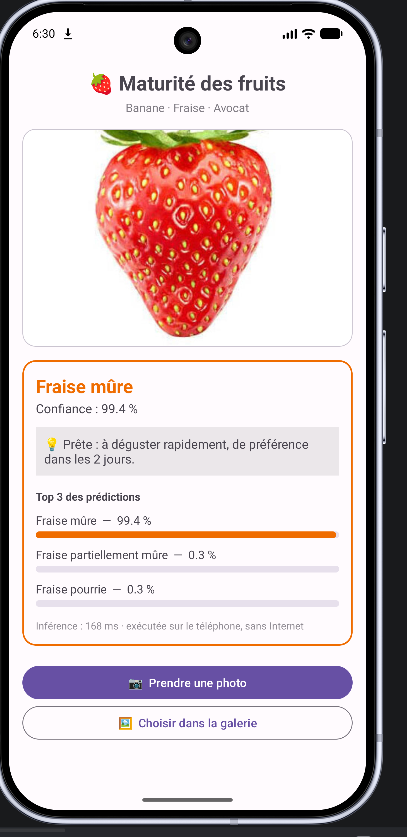
\includegraphics[height=7.0cm]{figures/app_fraise.png} &
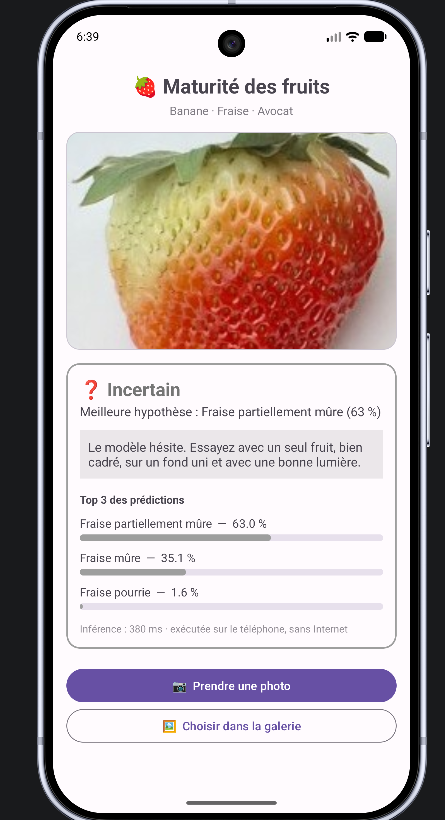
\includegraphics[height=7.0cm]{figures/app_fraise_incertain.png} &
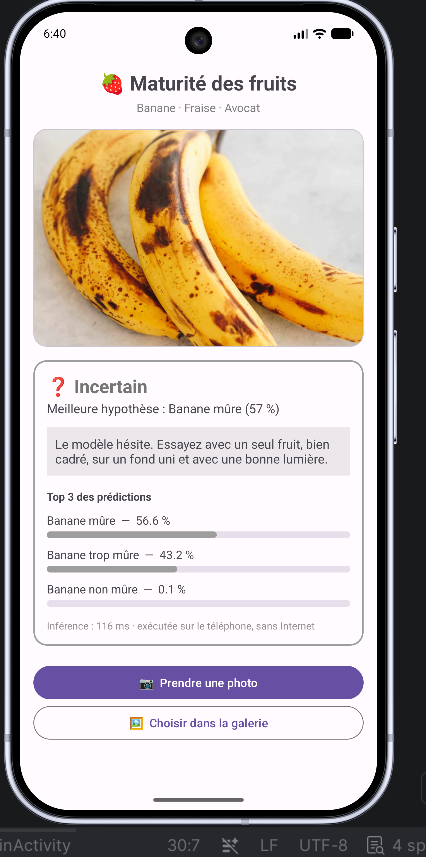
\includegraphics[height=7.0cm]{figures/app_bananes_incertain.png} &
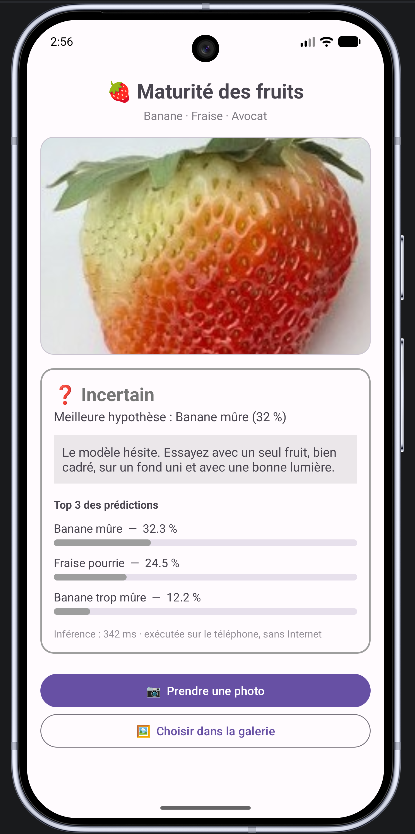
\includegraphics[height=7.0cm]{figures/app_cas.png} \\
{\scriptsize (a)} & {\scriptsize (b)} & {\scriptsize (c)} & {\scriptsize (d)}
\end{tabular}
\caption{Captures de l’application~: (a) fraise mûre reconnue avec 99,4\,\% de confiance ; (b) fraise à 63\,\%, marquée « Incertain » ; (c) bananes à 57\,\%, « Incertain » ; (d) fraise partiellement mûre d’une photo web : le meilleur score (32\,\%) va à « Banane mûre » et l’application déclare l’image incertaine.}\label{fig:captures}
\end{figure}

\begin{itemize}
  \item Dans le cas (a), un fruit isolé, bien éclairé, est reconnu à 99,4\,\% en 168\,ms.
  \item Dans les cas (b) et (c), le fruit est reconnu mais avec une confiance sous le seuil~: l’application évite d’affirmer et suggère de reprendre la photo.
  \item Le cas (d) est le plus instructif~: une fraise partiellement mûre photographiée dans un contexte très différent des données d’entraînement met le modèle en difficulté (un mauvais fruit en tête, avec 32\,\% seulement). Sans le seuil de confiance, l’application aurait annoncé « Banane mûre » ; c’est précisément le rôle de la classe « Incertain ».
\end{itemize}

\section{Points d’attention techniques}

\begin{itemize}
  \item \textbf{Orientation des photos}~: sans prise en compte de l’orientation EXIF, une photo prise en portrait serait analysée couchée. \code{ImageDecoder} règle ce point.
  \item \textbf{Qualité de la photo}~: la capture en pleine résolution passe par un \code{FileProvider}, qui donne à l’appareil photo du système le droit d’écrire dans un fichier privé de l’application.
  \item \textbf{Mémoire}~: les photos modernes (12 millions de pixels et plus) saturent la mémoire si on les décode entièrement~; d’où la limite à 1\,024 pixels.
  \item \textbf{Cohérence modèle/application}~: l’ordre des étiquettes et l’échelle des pixels (0--255) doivent correspondre exactement à ceux de l’entraînement.
  \item \textbf{Hors distribution}~: un objet qui n’est pas un fruit est tout de même classé. Le seuil limite le problème sans le supprimer (voir chapitre~\ref{chap:discussion}).
\end{itemize}

\section{Limites de l’application}

L’application suppose \textbf{un seul fruit par image}, car le modèle est un classifieur et non un détecteur. Elle ne gère que trois fruits et onze stades. Les tests ont été faits sur émulateur et sur quelques photos~; une campagne de tests sur plusieurs téléphones physiques n’a pas été réalisée.

\chapter{Discussion, limites et perspectives}\label{chap:discussion}

Ce chapitre prend du recul sur les résultats~: ce qu’ils démontrent, ce qu’ils ne démontrent pas, et ce qu’il faudrait faire pour aller plus loin.

\section{Ce que montrent les résultats}

Le transfert d’apprentissage avec MobileNetV2 permet d’atteindre une exactitude d’environ 93\,\% sur onze classes avec seulement 1\,118 images d’entraînement, en quelques minutes de calcul sur GPU. La quantification divise la taille du modèle par neuf sans perte significative, et le résultat tourne sur téléphone en quelques dizaines à quelques centaines de millisecondes. Le fruit est toujours correctement identifié ; les erreurs concernent des stades voisins, c’est-à-dire des cas où même des humains peuvent hésiter.

Les expériences négatives sont aussi instructives que les réussites~: une augmentation plus agressive et l’ajout de données d’une autre source n’ont pas amélioré, et ont même dégradé, les performances. Ce n’est pas un échec du projet mais un résultat~: le facteur limitant n’est pas la capacité du modèle, c’est la quantité et la cohérence des données étiquetées.

\section{Limites}

\paragraph{Taille du jeu de test.} Avec 231 images, l’intervalle de confiance à 95\,\% de l’exactitude s’étend de 89,0 à 95,7\,\%. Les classes de fraises comptent 6 à 14 images de test : leurs scores individuels sont très bruités, et il serait imprudent de conclure à une supériorité réelle d’un fruit sur l’autre à partir d’un écart de quelques images.

\paragraph{Subjectivité des étiquettes.} La maturité est un continuum découpé en classes par des annotateurs. La frontière entre «~partiellement mûr~» et «~mûr~» ou entre «~mûr~» et «~trop mûr~» dépend de l’opinion de la personne qui étiquette, comme le montre l’expérience 4. Un modèle ne peut pas être plus fiable que les étiquettes qui lui ont servi d’exemple.

\paragraph{Représentativité des photos.} Les images viennent de deux jeux publics, avec des fonds, des éclairages et des appareils particuliers. Le cas (d) du chapitre~\ref{chap:android} montre qu’une photo prise dans un contexte différent peut déstabiliser le modèle. Les performances mesurées s’appliquent à des images comparables à celles du test, pas nécessairement à toute photo prise par un utilisateur.

\paragraph{Un seul fruit par image.} Le modèle est un classifieur~: il décrit l’image entière. Une image contenant plusieurs fruits de stades différents, ou un fruit entouré de décor, sera mal traitée. Le recadrage par boîtes utilisé à l’entraînement n’existe pas à l’usage~: c’est à l’utilisateur de cadrer le fruit.

\paragraph{Objets hors du domaine.} Le softmax attribue toujours des probabilités à 11 classes, même pour un objet qui n’est pas un fruit. Le seuil de confiance atténue le problème sans le résoudre~: un objet peut recevoir une forte probabilité sur une classe.

\paragraph{Calibration des probabilités.} Le seuil de 70\,\% est fixé de façon empirique. Les probabilités d’un réseau profond sont souvent trop confiantes ; nous n’avons pas mesuré la calibration (par exemple avec la courbe de fiabilité).

\paragraph{Tests de l’application.} L’application a été testée sur un émulateur et quelques photos. Les temps d’inférence réels sur des téléphones physiques, et le comportement sur des appareils variés (mémoire, orientation, caméras) restent à mesurer.

\paragraph{Usage et responsabilité.} L’application donne des repères de consommation («~à consommer dans les 1 à 2 jours~»). Elle n’est pas un outil de sécurité alimentaire~: pour un fruit visiblement abîmé ou moisi, le conseil de prudence reste prioritaire, et la décision revient à l’utilisateur.

\section{Perspectives}

\begin{table}[H]
\centering
\caption{Pistes d’amélioration et bénéfice attendu.}\label{tab:persp}
\small
\begin{tabularx}{\textwidth}{@{}p{4.1cm}X@{}}
\toprule
\textbf{Piste} & \textbf{Bénéfice attendu} \\
\midrule
Données supplémentaires avec une convention d’étiquetage unique & Améliorer les classes rares (fraises, avocat mûr) sans l’incohérence observée à l’expérience 4 \\
Validation croisée sur les photos d’origine & Réduire l’incertitude de la mesure malgré le petit effectif \\
Classe «~autre~» ou détection de nouveauté & Refuser les objets qui ne sont pas des fruits \\
Étalonnage des probabilités (\emph{temperature scaling}) & Rendre le seuil de confiance plus fiable \\
Détecteur de fruits (YOLO) puis classifieur & Traiter plusieurs fruits par image, sans cadrage manuel \\
Régression ordinale de la maturité & Respecter l’ordre des stades et pénaliser davantage les grandes erreurs \\
Quantification entière complète, délégué GPU & Réduire la latence et la consommation sur téléphone \\
Tests sur plusieurs téléphones physiques & Mesurer les temps réels et la robustesse de la capture \\
Autres fruits et variétés & Élargir l’utilité de l’application \\
\bottomrule
\end{tabularx}
\end{table}

L’une des pistes les plus prometteuses est le \textbf{traitement ordinal} de la maturité. Les classes sont ordonnées (non mûr $<$ partiellement mûr $<$ mûr $<$ pourri), mais l’entropie croisée traite toutes les erreurs de la même manière~: confondre «~non mûr~» et «~pourri~» coûte autant que confondre deux stades voisins. Une perte ordinale, ou une régression d’un indice de maturité continu, reflèterait mieux la réalité du problème.

\chapter*{Conclusion générale}
\addcontentsline{toc}{chapter}{Conclusion générale}
\thispagestyle{plain}

Ce projet avait pour but de concevoir un système capable de reconnaître, sur un smartphone et sans connexion, le fruit et son stade de maturité à partir d’une simple photographie. Nous y sommes parvenus de bout en bout~: de la préparation des données au déploiement dans une application Android fonctionnelle.

Sur le plan théorique, nous avons rappelé les bases du deep learning, détaillé le fonctionnement des réseaux convolutifs (convolution, pooling, normalisation par lots) et expliqué ce qui fait la légèreté de MobileNet~: la convolution séparable en profondeur, qui réduit le coût d’un facteur proche de neuf, et le bloc résiduel inversé à goulot linéaire de MobileNetV2.

Sur le plan expérimental, un modèle MobileNetV2 affiné en deux phases atteint \textbf{93,1\,\%} d’exactitude sur un jeu de test de 231 images (intervalle de confiance à 95\,\% : 89,0 à 95,7\,\%), avec un F1 macro de 0,90. Il identifie toujours correctement le fruit ; ses erreurs se situent entre stades voisins. La quantification dynamique ramène le modèle de 23,1 à \textbf{2,5\,Mo} pour une perte d’une seule image sur 231, avec un temps d’inférence de l’ordre de 20\,ms sur CPU.

Sur le plan applicatif, l’application Android exécute le modèle localement, corrige l’orientation des photos, moyenne les prédictions sur l’image et son miroir, et surtout \emph{s’abstient de répondre} quand elle n’est pas sûre~: un seuil de confiance de 70\,\% déclenche les mentions « Incertain » ou « entre deux stades ». Chaque résultat s’accompagne d’un conseil pratique.

Le projet nous a aussi enseigné plusieurs leçons méthodologiques. Découper les données par photo d’origine évite une évaluation trop optimiste~; réutiliser sans précaution des objets de rappel (\emph{callbacks}) entre deux phases d’entraînement peut dégrader silencieusement les résultats~; geler les couches de normalisation en fine-tuning est déterminant~; enfin, ajouter des données d’une autre source n’aide que si les étiquettes suivent la même convention, comme le montre notre expérience sur les bananes.

Les limites sont claires~: un jeu de test de taille modeste, des étiquettes de maturité subjectives, un seul fruit par image, aucune détection des objets qui ne sont pas des fruits et des tests limités à un émulateur. Les perspectives les plus directes sont l’enrichissement des données avec une convention d’étiquetage unique, l’étalonnage des probabilités, un détecteur de fruits en amont du classifieur et une mesure sur plusieurs téléphones réels.

Au-delà de ce cas particulier, ce travail illustre une idée simple~: grâce au transfert d’apprentissage et à la quantification, un réseau profond utile peut aujourd’hui tenir dans quelques mégaoctets et s’exécuter dans la poche de l’utilisateur, sans que ses photos ne quittent son téléphone.

\chapter*{Références}
\addcontentsline{toc}{chapter}{Références}
\thispagestyle{plain}

\begin{thebibliography}{99}
\small
\setlength{\itemsep}{3pt}

\bibitem{goodfellow2016} I.~Goodfellow, Y.~Bengio et A.~Courville, \emph{Deep Learning}, MIT Press, 2016.

\bibitem{kingma2015} D.~P.~Kingma et J.~Ba, «~Adam: A Method for Stochastic Optimization~», \emph{International Conference on Learning Representations (ICLR)}, 2015.

\bibitem{srivastava2014} N.~Srivastava, G.~Hinton, A.~Krizhevsky, I.~Sutskever et R.~Salakhutdinov, «~Dropout: A Simple Way to Prevent Neural Networks from Overfitting~», \emph{Journal of Machine Learning Research}, vol.~15, p.~1929--1958, 2014.

\bibitem{ioffe2015} S.~Ioffe et C.~Szegedy, «~Batch Normalization: Accelerating Deep Network Training by Reducing Internal Covariate Shift~», \emph{International Conference on Machine Learning (ICML)}, 2015.

\bibitem{lecun1998} Y.~LeCun, L.~Bottou, Y.~Bengio et P.~Haffner, «~Gradient-Based Learning Applied to Document Recognition~», \emph{Proceedings of the IEEE}, vol.~86, n$^\circ$~11, p.~2278--2324, 1998.

\bibitem{krizhevsky2012} A.~Krizhevsky, I.~Sutskever et G.~E.~Hinton, «~ImageNet Classification with Deep Convolutional Neural Networks~», \emph{Advances in Neural Information Processing Systems (NeurIPS)}, vol.~25, 2012.

\bibitem{simonyan2015} K.~Simonyan et A.~Zisserman, «~Very Deep Convolutional Networks for Large-Scale Image Recognition~», \emph{ICLR}, 2015.

\bibitem{he2016} K.~He, X.~Zhang, S.~Ren et J.~Sun, «~Deep Residual Learning for Image Recognition~», \emph{IEEE Conference on Computer Vision and Pattern Recognition (CVPR)}, 2016.

\bibitem{howard2017} A.~G.~Howard \emph{et al.}, «~MobileNets: Efficient Convolutional Neural Networks for Mobile Vision Applications~», \emph{arXiv:1704.04861}, 2017.

\bibitem{sandler2018} M.~Sandler, A.~Howard, M.~Zhu, A.~Zhmoginov et L.-C.~Chen, «~MobileNetV2: Inverted Residuals and Linear Bottlenecks~», \emph{CVPR}, 2018.

\bibitem{deng2009} J.~Deng, W.~Dong, R.~Socher, L.-J.~Li, K.~Li et L.~Fei-Fei, «~ImageNet: A Large-Scale Hierarchical Image Database~», \emph{CVPR}, 2009.

\bibitem{yosinski2014} J.~Yosinski, J.~Clune, Y.~Bengio et H.~Lipson, «~How Transferable Are Features in Deep Neural Networks?~», \emph{NeurIPS}, vol.~27, 2014.

\bibitem{jacob2018} B.~Jacob \emph{et al.}, «~Quantization and Training of Neural Networks for Efficient Integer-Arithmetic-Only Inference~», \emph{CVPR}, 2018.

\bibitem{redmon2016} J.~Redmon, S.~Divvala, R.~Girshick et A.~Farhadi, «~You Only Look Once: Unified, Real-Time Object Detection~», \emph{CVPR}, 2016.

\bibitem{dib2025} «~Comprehensive Dataset on Ripening Stages of Strawberries and Avocados From Unripe to Rotten~», \emph{Data in Brief}, 2025. Jeu de données public d’images annotées au format YOLO.

\bibitem{banane_ds} «~Banana Ripeness Dataset~»~: images de bananes à trois stades de maturité (non mûre, mûre, trop mûre) annotées au format YOLO. Jeu de données public.

\bibitem{docs} Documentation officielle~: \emph{Keras Applications} (\url{https://keras.io/api/applications/}), \emph{TensorFlow Lite} (\url{https://www.tensorflow.org/lite}) et \emph{Android Developers} (\url{https://developer.android.com}).

\end{thebibliography}

\appendix

\chapter{Code d’entraînement (extraits)}\label{app:code}

Les extraits ci-dessous reprennent la structure du carnet d’entraînement. La construction du modèle est reconstituée à partir de la configuration enregistrée du modèle retenu (augmentation, dropout, tête de classification)~; les valeurs des phases d’entraînement sont celles décrites au chapitre~\ref{chap:modele}.

\Needspace*{12\baselineskip}
\section{Construction du modèle}

\begin{lstlisting}[language=PythonK]
IMG, N = (224, 224), 11

augment = tf.keras.Sequential([
    tf.keras.layers.RandomFlip("horizontal_and_vertical"),
    tf.keras.layers.RandomRotation(0.15),
    tf.keras.layers.RandomZoom(0.15),
    tf.keras.layers.RandomBrightness(0.1),
    tf.keras.layers.RandomContrast(0.1),
], name="augmentation")      # pas de changement de teinte

base = tf.keras.applications.MobileNetV2(
    input_shape=IMG + (3,), include_top=False, weights="imagenet")
base.trainable = False       # phase 1 : base gelee

inputs = tf.keras.Input(shape=IMG + (3,))        # pixels 0-255
x = augment(inputs)
x = tf.keras.applications.mobilenet_v2.preprocess_input(x)   # [-1,1]
x = base(x, training=False)
x = tf.keras.layers.GlobalAveragePooling2D()(x)
x = tf.keras.layers.Dropout(0.3)(x)
outputs = tf.keras.layers.Dense(N, activation="softmax")(x)
model = tf.keras.Model(inputs, outputs)
\end{lstlisting}

\Needspace*{12\baselineskip}
\section{Poids de classes et phase 1}

\begin{lstlisting}[language=PythonK]
y_train = np.concatenate([y.numpy() for _, y in train_ds])
weights = compute_class_weight("balanced",
                               classes=np.arange(N), y=y_train)
CLASS_WEIGHT = dict(enumerate(weights))

cb1 = [tf.keras.callbacks.EarlyStopping(monitor="val_loss", patience=6,
                                        restore_best_weights=True),
       tf.keras.callbacks.ReduceLROnPlateau(monitor="val_loss",
                                            factor=0.5, patience=3)]
model.compile(optimizer=tf.keras.optimizers.Adam(1e-3),
              loss="sparse_categorical_crossentropy",
              metrics=["accuracy"])
hist1 = model.fit(train_ds, validation_data=val_ds, epochs=25,
                  class_weight=CLASS_WEIGHT, callbacks=cb1)
\end{lstlisting}

\Needspace*{12\baselineskip}
\section{Phase 2~: fine-tuning}

\begin{lstlisting}[language=PythonK]
base.trainable = True
FREEZE_UNTIL = len(base.layers) - 40          # 40 dernieres couches
for i, layer in enumerate(base.layers):
    layer.trainable = (i >= FREEZE_UNTIL) and not isinstance(
        layer, tf.keras.layers.BatchNormalization)

cb2 = [tf.keras.callbacks.EarlyStopping(monitor="val_loss", patience=10,
                                        restore_best_weights=True),
       tf.keras.callbacks.ReduceLROnPlateau(monitor="val_loss", factor=0.5,
                                            patience=4, min_lr=1e-7)]
model.compile(optimizer=tf.keras.optimizers.Adam(1e-5),
              loss="sparse_categorical_crossentropy",
              metrics=["accuracy"])
hist2 = model.fit(train_ds, validation_data=val_ds, epochs=40,
                  class_weight=CLASS_WEIGHT, callbacks=cb2)
\end{lstlisting}

Remarque~: les objets \code{cb1} et \code{cb2} sont créés séparément~; réutiliser les mêmes callbacks dans les deux phases conserverait en mémoire la meilleure perte de la phase 1 (section~\ref{sec:finetune}).

\chapter{Code de l’application Android (extraits)}\label{app:kotlin}

\Needspace*{12\baselineskip}
\section{Inférence avec test-time augmentation}

\begin{lstlisting}[language=Kotlin]
/** Probabilités des 11 classes, moyennées sur l'image et son miroir. */
private fun classify(bitmap: Bitmap): FloatArray {
    val src = bitmap.copy(Bitmap.Config.ARGB_8888, false)
    val flipped = Bitmap.createBitmap(
        src, 0, 0, src.width, src.height,
        Matrix().apply { preScale(-1f, 1f) }, true)
    val a = runModel(Bitmap.createScaledBitmap(src, IMG_SIZE, IMG_SIZE, true))
    val b = runModel(Bitmap.createScaledBitmap(flipped, IMG_SIZE, IMG_SIZE, true))
    return FloatArray(a.size) { (a[it] + b[it]) / 2f }
}

private fun runModel(scaled: Bitmap): FloatArray {
    // Pixels RGB float32 entre 0 et 255 (normalisation dans le modèle)
    val input = ByteBuffer.allocateDirect(4 * IMG_SIZE * IMG_SIZE * 3)
        .order(ByteOrder.nativeOrder())
    val pixels = IntArray(IMG_SIZE * IMG_SIZE)
    scaled.getPixels(pixels, 0, IMG_SIZE, 0, 0, IMG_SIZE, IMG_SIZE)
    for (p in pixels) {
        input.putFloat(((p shr 16) and 0xFF).toFloat())  // R
        input.putFloat(((p shr 8) and 0xFF).toFloat())   // G
        input.putFloat((p and 0xFF).toFloat())           // B
    }
    input.rewind()
    val output = Array(1) { FloatArray(labels.size) }
    interpreter.run(input, output)
    return output[0]
}
\end{lstlisting}

\Needspace*{12\baselineskip}
\section{Décision~: fiable, entre deux stades ou incertain}

\begin{lstlisting}[language=Kotlin]
val top = probs.withIndex().sortedByDescending { it.value }.take(3)
val best = labels[top[0].index]
val conf = top[0].value
val uncertain = conf < CONFIDENCE_MIN            // 0.70

val second = labels[top[1].index]
val sameFruit = best.substringBefore("_") == second.substringBefore("_")
val between = uncertain && sameFruit && (conf + top[1].value) >= 0.85f

if (between) {
    // deux stades voisins du même fruit se partagent le résultat
} else if (uncertain) {
    // "Incertain" : meilleure hypothèse donnée à titre indicatif
} else {
    // résultat fiable : classe, confiance et conseil
}
\end{lstlisting}

\chapter{Résultats détaillés}\label{app:resultats}

\Needspace*{12\baselineskip}
\section{Classes et ordre des sorties}

L’ordre des 11 sorties du modèle (fichier \code{labels.txt}) est l’ordre alphabétique suivant~:

\begin{enumerate}[nosep,leftmargin=*]
  \item \code{avocat\_mur}
  \item \code{avocat\_non\_mur}
  \item \code{avocat\_partiellement\_mur}
  \item \code{avocat\_pourri}
  \item \code{banane\_mure}
  \item \code{banane\_non\_mure}
  \item \code{banane\_trop\_mure}
  \item \code{fraise\_mure}
  \item \code{fraise\_non\_mure}
  \item \code{fraise\_partiellement\_mure}
  \item \code{fraise\_pourrie}
\end{enumerate}

\Needspace*{12\baselineskip}
\section{Rappel des chiffres clés}

\begin{table}[H]
\centering
\caption{Chiffres clés du projet.}\label{tab:cles}
\small
\begin{tabular}{@{}lr@{}}
\toprule
\textbf{Grandeur} & \textbf{Valeur} \\
\midrule
Photographies d’origine & 1\,431 \\
Images de fruits recadrées & 1\,598 \\
Entraînement / validation / test & 1\,118 / 249 / 231 \\
Paramètres du modèle & 2\,272\,075 \\
Exactitude de test (Keras) & 93,07\,\% (215/231) \\
Intervalle de Wilson à 95\,\% & [89,0\,\% ; 95,7\,\%] \\
F1 macro & 0,897 \\
Exactitude de test (TFLite quantifié) & 92,64\,\% (214/231) \\
Taille Keras / TFLite & 23,1\,Mo / 2,5\,Mo \\
Inférence CPU (Kaggle) & 19,6\,ms \\
\bottomrule
\end{tabular}
\end{table}


\end{document}
